\documentclass[twocolumn]{article}
\usepackage{amsmath,amsfonts}
\usepackage{algorithmic}
\usepackage{algorithm}
\usepackage{array}
\usepackage[caption=false,font=normalsize,labelfont=sf,textfont=sf]{subfig}
\usepackage{textcomp}
\usepackage{stfloats}
\usepackage{url}
\usepackage{verbatim}
\usepackage{graphicx}
\usepackage{cite}
\usepackage[hidelinks]{hyperref}
\usepackage{booktabs}
\usepackage{multirow}
\hyphenation{}

% 修改处采用 \rev{} 包裹，下面 \newcommand 两个二选一，要注释掉另一个
\usepackage{xcolor}
% \newcommand{\rev}[1]{\textcolor{blue}{#1}} % 生成带标注的 marked version
\newcommand{\rev}[1]{#1} % 生成不带标注的正常版本 clean version

\begin{document}

\title{MAT4PM: Machine Learning-Guided Adaptive Threshold Control\\
for P4-based Monitoring in SDNs}

\author{
    Henghua Zhang,
    Jue Chen, 
    Haidong Peng, 
    and Junru Chen
    \thanks{
        The authors are with the School of Electronic and Electrical Engineering, 
        Shanghai University of Engineering Science, 
        Shanghai 201620, China 
        (e-mail: \href{mailto:zhang@sues.edu.cn}{zhang@sues.edu.cn}; 
                 \href{mailto:jadeschen@sues.edu.cn}{jadeschen@sues.edu.cn}; 
                 \href{mailto:m325124607@sues.edu.cn}{m325124607@sues.edu.cn}; 
                 \href{mailto:m325124267@sues.edu.cn}{m325124267@sues.edu.cn}). 
        \textit{(Corresponding author: Jue Chen.)}
    }
}

\date{}

\maketitle

\begin{center}
\footnotesize{\copyright~IEEE. Personal use of this material is permitted.\\
For other uses, permission must be obtained from IEEE.}
\end{center}

\noindent
This is the author’s version of a work accepted for publication in 
\textit{IEEE Transactions on Network and Service Management}.  
The final version is available at IEEE Xplore:
\url{https://doi.org/10.1109/TNSM.2026.3677416}

\begin{abstract}
    This paper presents MAT4PM, a P4-based proactive monitoring framework designed for Software-Defined Networking (SDN). 
    % To the best of our knowledge, this is the first monitoring framework to jointly leverage programmable data plane capabilities for event-driven data collection and control plane intelligence for real-time threshold optimization. 
    \rev{This is the first monitoring framework that combines Programmable Data Plane (PDP) capabilities for event-driven data collection with control plane intelligence for real-time threshold optimization.} 
    % The system architecture comprises a lightweight P4-based monitoring module deployed at the switch, a machine learning inference engine operating at the controller, and a P4Runtime feedback channel for real-time threshold updates. 
    \rev{The architecture consists of a lightweight P4-based monitoring module deployed at the switch, a Machine Learning (ML) inference engine running at the controller, and a P4Runtime feedback channel for real-time threshold updates.} 
    % The framework leverages traffic features to predict optimal monitoring thresholds, which are subsequently synchronized to the data plane. 
    \rev{Traffic features are leveraged to predict optimal monitoring thresholds, which are then synchronized with the data plane.}
    % A composite cost function is introduced, jointly considering monitoring error and communication overhead, to guide the model toward a balanced trade-off between accuracy and efficiency. 
    \rev{A composite cost function is introduced to jointly consider monitoring error and communication overhead, guiding the model toward a balanced trade-off between accuracy and efficiency.}
    Experimental evaluation on BMv2 software switches demonstrates that, compared to static threshold strategies, MAT4PM reduces monitoring error to 7.0\% and achieves a 5.6\% reduction in overall cost, while maintaining sub-millisecond inference latency and minimal resource consumption. 
    % These results indicate strong practical viability and scalability for real-world SDN environments.
    \rev{These results demonstrate the practical viability and scalability of MAT4PM in SDN environments.}
\end{abstract}

\noindent \textbf{Keywords:} 
Software-Defined Networking, 
Programmable Data Plane, 
Machine Learning, 
Network Monitoring, 
P4

\section{Introduction}

With the continuous expansion of network scale and complexity, traditional network architectures are increasingly challenged in terms of flexibility, scalability, and automated management. 
Software-Defined Networking (SDN)~\cite{JANG2023105736} has emerged as a novel architectural paradigm that decouples the control plane from the data plane, enabling centralized management and flexible configuration of network resources~\cite{9360650}. 
While SDN's centralized control plane enables dynamic network orchestration through protocols such as OpenFlow~\cite{10.1145/1355734.1355746}, effective management depends not merely on rule deployment but also on real-time state awareness. 
% Accurate and timely acquisition of network states is thus indispensable, underscoring monitoring as a fundamental SDN capability~\cite{10.1145/3556973}.
\rev{Accurate and timely acquisition of network states is essential, making monitoring a fundamental SDN capability~\cite{10.1145/3556973}.}

SDN switches inherently support the collection of flow-level statistics such as packet counts, byte volumes, and flow duration, providing a foundation for fine-grained traffic monitoring \cite{KALAMBE2025104081}. Existing monitoring mechanisms primarily fall into two categories: push-based \cite{10.1145/3373360.3380830, 6888899, 10.1007/978-3-642-36516-4_4} and pull-based \cite{7037094, CASTILLO2020107108, 8411125, 10.1007/978-3-642-12334-4_21} approaches. 
Push-based schemes periodically or event-drivenly transmit flow statistics to the controller, offering better timeliness but often leading to congestion in the control channel and excessive load on the controller. 
In contrast, pull-based schemes rely on the controller to actively request statistics, offering greater flexibility but suffering from trade-offs between accuracy and overhead: short polling intervals increase system burden, while longer intervals risk delayed anomaly detection. 
Moreover, in either case, the centralized accumulation of monitoring data at the controller may introduce performance bottlenecks, undermining critical tasks such as route computation and flow table updates \cite{8291608}.

The advent of data plane programmability, particularly with the rise of the P4 (Programming Protocol-Independent Packet Processors) language~\cite{10.1145/2656877.2656890}, has revolutionized traffic monitoring in SDN. 
P4 enables protocol-agnostic and behavior-customized packet processing, allowing switches to implement more flexible and efficient data collection strategies \cite{HAUSER2023103561}. 
For instance, by embedding lightweight filtering or labeling logic within the switch pipeline, non-essential data can be preprocessed and discarded locally, thereby reducing the volume of traffic forwarded to the controller and alleviating pressure on the control plane \cite{10130445}. 
Nonetheless, designing a monitoring mechanism that achieves high accuracy with low overhead under a programmable data plane (PDP)~\cite{PDP} architecture remains an open and challenging problem \cite{KAUR2021109}.

Meanwhile, Machine Learning (ML) has shown considerable promise in network management, particularly in behavior modeling of complex systems, anomaly detection, and policy optimization \cite{JAMSHIDI2025111103, JISI2025110939, Serag2025, 10480735, 10273389, 10198239, FOSIC2023100466, 9505258}. 
In the context of SDN monitoring, ML-based approaches can assist the controller in dynamically adjusting monitoring policies under uncertain or time-varying traffic conditions---e.g., by selectively sampling flows \cite{9335605}---thus improving the balance between monitoring accuracy and system overhead. 
Although prior works have investigated Reinforcement Learning (RL)~\cite{RL}, Supervised Learning (SL)~\cite{SupervisedLearning}, or Federated Learning (FL)~\cite{FL} for optimizing monitoring policies, few have fully leveraged the programmability offered by P4 to jointly optimize the trade-off between control overhead and monitoring precision from both the data and control planes \cite{SONI2022103419}. 
% As far as is known, this is the first paper to propose an SDN monitoring framework that explicitly integrates programmable data plane mechanisms enabled by P4 with machine learning-based adaptive policy inference on the control plane. 
\rev{This paper presents the first SDN monitoring framework that integrates P4-enabled programmable data plane mechanisms with machine learning-based adaptive policy inference on the control plane.} 
This cross-plane coordination enables closed-loop, fine-grained monitoring with improved adaptability and efficiency. 
Based on this architectural principle, a framework named MAT4PM (Machine Learning-Guided Adaptive Threshold Control for P4-based Monitoring) is developed. 
It integrates event-driven monitoring logic implemented in the P4 data plane with predictive threshold adjustment conducted by control-plane machine learning models~\cite{MAT4PM}. 
The primary contributions are summarized as follows:

\begin{enumerate}
    
    \item A collaborative monitoring mechanism is designed and implemented by combining P4-based active reporting at the data plane with machine learning-driven policy tuning at the control plane. 
    Building upon the advantages of proactive schemes such as PPM (P4-based Proactive Monitoring) \cite{10623873}, the proposed approach eliminates the reliance on manually configured thresholds by dynamically predicting monitoring intervals through learned models with real-time traffic features as input. 
    The system establishes a closed-loop architecture characterized by data plane event triggering and control plane intelligent decision-making, thereby achieving high accuracy, low overhead, and strong adaptability under dynamic traffic scenarios.
    
    \item A data construction methodology is formulated to support optimal threshold learning and facilitate the generation of a high-quality labeled dataset. 
    Optimal thresholds are derived from offline simulations that minimize a jointly defined cost function, serving as ground truth labels for supervised learning. 
    Packet trace files (pcap)~\cite{pcap} captured from the BMv2 switch under various monitoring intervals are replayed to quantify estimation errors and communication overheads.
    
    \item A full prototype system is developed, comprising P4-based data plane logic, controller-side decision modules, and three mainstream machine learning models---eXtreme Gradient Boosting (XGBoost)~\cite{XGBoost}, Light Gradient Boosting Machine (LightGBM)~\cite{LightGBM}, and Support Vector Machine (SVM)~\cite{SVM}. 
    Experimental results demonstrate that, compared to fixed-threshold schemes, the proposed dynamic adjustment mechanism reduces the average estimation error from 9.1\% to 7.0\% and lowers the overall monitoring cost by 5.6\%. 
    In addition, the models exhibit low prediction latency (all below 5~ms) and minimal resource consumption (memory usage: 13.89 KB-36.24 KB), indicating the feasibility of real-time deployment in operational environments.
    
\end{enumerate}

% \rev{The terminology and abbreviations used throughout this paper are summarized in Table~\ref{tab:acronyms} for reference.} 
The remainder of this paper is organized as follows. Section~\ref{sec2} reviews background and related work, including fundamental concepts of programmable data planes and existing P4-based monitoring approaches. Section~\ref{sec3} details the architecture and core components of the proposed MAT4PM system. Section~\ref{sec4} presents experimental evaluations to validate the effectiveness of our method. Section~\ref{sec5} concludes the paper and discusses potential future research directions.

% \begin{table}[!t]
%     \centering
%     \caption{\rev{List of Acronyms and Definitions}}
%     \label{tab:acronyms}
%     \begin{tabular}{p{0.09\textwidth} p{0.35\textwidth}}
%         \toprule
%         \multirow{1}{=}{\textbf{Abbreviation}} & \textbf{Definition} \\
%         \midrule
%         \rev{API} & \rev{Application Programming Interface} \\
%         \rev{ASIC} & \rev{Application-Specific Integrated Circuit} \\
%         \rev{BMv2} & \rev{Behavioral Model version 2} \\
%         \rev{BPS} & \rev{Bits Per Second} \\
%         \rev{CI} & \rev{Confidence Interval} \\
%         \rev{CPU} & \rev{Central Processing Unit} \\
%         \rev{DLINT} & \rev{Deterministic Lightweight In-Band Network Telemetry} \\
%         \rev{DPDK} & \rev{Data Plane Development Kit} \\
%         \rev{FL} & \rev{Federated Learning} \\
%         \rev{FS-INT} & \rev{Flexible Sampling-based In-band Network Telemetry} \\
%         \rev{INT} & \rev{In-band Network Telemetry} \\
%         \rev{INTO} & \rev{In-band Network Telemetry Orchestration} \\
%         \rev{LightGBM} & \rev{Light Gradient Boosting Machine} \\
%         \rev{LB} & \rev{Load Balancing} \\
%         \rev{MAC} & \rev{Media Access Control} \\
%         \rev{MSE} & \rev{Mean Squared Error} \\
%         \rev{ML} & \rev{Machine Learning} \\
%         \rev{OVS} & \rev{Open vSwitch} \\
%         \rev{P4} & \rev{Programming Protocol-independent Packet Processor} \\
%         \rev{PCAP} & \rev{Packet Capture} \\
%         \rev{PDP} & \rev{Programmable Data Plane} \\
%         \rev{PLINT} & \rev{Probabilistic Lightweight In-Band Network Telemetry} \\
%         \rev{PPM} & \rev{P4-based Proactive Monitoring} \\
%         \rev{PPS} & \rev{Packets Per Second} \\
%         \rev{RAM} & \rev{Random Access Memory} \\
%         \rev{RL} & \rev{Reinforcement Learning} \\
%         \rev{RPC} & \rev{Remote Procedure Call} \\
%         \rev{Std. Dev.} & \rev{Standard Deviation} \\
%         \rev{SDN} & \rev{Software-defined Networking} \\
%         \rev{SL} & \rev{Supervised Learning} \\
%         \rev{SVM} & \rev{Support Vector Machine} \\
%         \rev{TCP} & \rev{Transmission Control Protocol} \\
%         \rev{TBSW} & \rev{Time-based Sliding Window} \\
%         \rev{UDP} & \rev{User Datagram Protocol} \\
%         \rev{VM} & \rev{Virtual Machine} \\
%         \rev{XGBoost} & \rev{eXtreme Gradient Boosting} \\
%         \bottomrule
%     \end{tabular}
% \end{table}

\section{Background and Related Work}
\label{sec2}

\subsection{Background}

\begin{figure*}[!t]
    \centering
    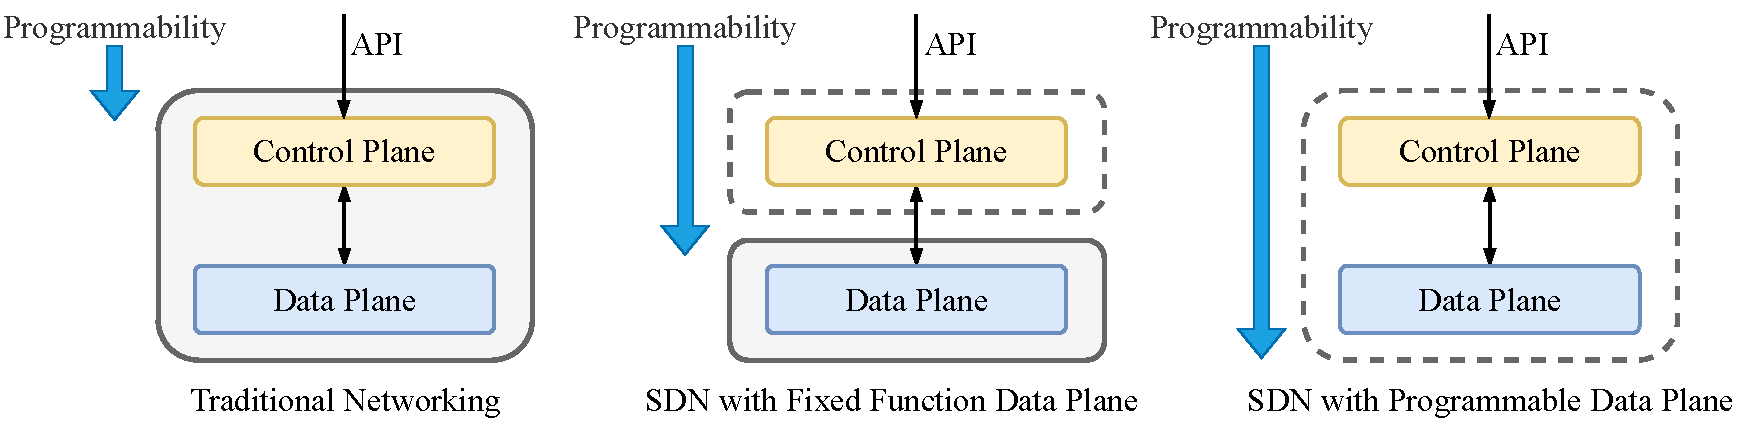
\includegraphics[width=0.85\textwidth]{./figures/evolution.pdf}
    \caption{Evolution of networks.}
    \label{evolution}
\end{figure*}

\noindent
% In recent years, network architectures have undergone a fundamental evolution, progressing from traditional distributed device management to centralized SDN, and further toward next-generation paradigms featuring programmable data planes. 
\rev{In recent years, network architectures have undergone a fundamental evolution, shifting from traditional distributed device management to centralized SDN, and further toward next-generation paradigms with programmable data planes.} 
This evolution is illustrated in Figure~\ref{evolution}. 
On the left of this figure, traditional network designs exhibit a tightly coupled relationship between the control logic and data forwarding processes. 
Network devices in this model are typically closed and inflexible, with static functions hardcoded by vendors. 
Updating policies requires manual intervention and device reconfiguration, significantly limiting the scalability and adaptability of the network. 
The middle part of the figure depicts the canonical SDN architecture, where the control plane is decoupled from individual network devices and centralized within the SDN controller(s). 
This architectural shift enables centralized policy management and dynamic control of network behavior, leading to substantial improvements in programmability and automation. However, this programmability is largely confined to the control plane. 
The data plane, constrained by static match-action rules, lacks the flexibility to respond rapidly and granularly to real-time traffic dynamics. 
The right part of the figure illustrates the integration of programmable data planes into SDN, marking a new phase in the evolution toward intelligent and highly customizable networks. 
By enabling programmability at the data plane, network devices can be redefined to support protocol-independent, state-aware, and fully customizable packet processing behaviors. 
This capability enhances the network's responsiveness to dynamic traffic patterns and significantly improves operational agility and efficiency.

A key technological milestone in this evolution is the emergence of the P4 language \cite{P4.org}, which plays a foundational role in the development of programmable data planes. 
P4 is a high-level, domain-specific language tailored for describing packet-processing behaviors. 
Its core design objective is to achieve protocol independence and flexible behavior specification within the data plane. 
% Using P4 programs, developers gain fine-grained control over the packet processing pipeline of a switch, including parsing, matching, modifying, and forwarding actions. 
\rev{P4 programs provide developers with fine-grained control over the packet processing pipeline of a switch, including parsing, matching, modifying, and forwarding actions.} 
This programmability not only extends the functional boundaries of network devices but also introduces new opportunities for building efficient and intelligent traffic monitoring systems. 
In particular, P4 facilitates the deployment of custom traffic classification and filtering mechanisms directly within the data plane. 
Developers can embed user-defined logic to monitor or tag only specific types of flows, thereby enabling preliminary state processing without relying on frequent controller intervention. 
Compared to traditional polling-based monitoring approaches, this architecture significantly reduces control plane communication overhead while improving response latency and system scalability.

\subsection{Related Work}

\noindent With the advancement of programmable data plane technologies, a variety of P4-based SDN traffic monitoring solutions have been proposed to improve the timeliness, accuracy, and scalability of network monitoring. 
Among them, In-band Network Telemetry (INT)~\cite{INT} represents a widely adopted monitoring framework. 
% The core idea of INT is to attach metadata to packet headers, which can be modified by intermediate switches along the forwarding path, enabling data plane state collection without controller intervention \cite{8094182, kim2015band}. 
\rev{The core idea of INT is to attach metadata to packet headers that are modified by intermediate switches along the forwarding path, enabling data plane state collection without controller intervention \cite{8094182, kim2015band}.} 
This mechanism allows switches to embed performance indicators such as latency and packet loss rate at each hop. 
The receiver subsequently extracts the full path metadata for comprehensive analysis. 
However, the additional headers introduced by INT result in significant protocol overhead, which increases sharply with path length and severely limits its practical applicability. 
To address this issue, researchers have developed several lightweight optimization strategies. 
For example, FS-INT \cite{SUH202062} proposes a flexible sampling mechanism that combines proportional and event-driven sampling to annotate only selected key packets with INT metadata. 
This approach retains essential monitoring capabilities while effectively controlling overhead, adapting to the performance requirements of diverse network environments. 
More recently, DLINT and PLINT \cite{10206040} have been proposed as deterministic and probabilistic enhancements to P4-INT. 
DLINT introduces per-flow telemetry state aggregation with Bloom filter-based compression, while PLINT adopts reservoir sampling to probabilistically embed telemetry information across packets. 
Both techniques significantly reduce overhead while preserving telemetry accuracy, offering complementary advantages in path trace reconstruction and update detection.

Beyond INT-based solutions, various active or distributed P4-enabled monitoring schemes have been developed. 
The network is partitioned into multiple monitoring domains by FlowStalker, where each domain collects local traffic information using specially crafted packets and periodically reports it to the controller \cite{8761197}. 
FlowSpy, in contrast, employs a load balancing mechanism to optimize communication between the data plane and controller, thereby enhancing monitoring efficiency \cite{8891487}. 
The work in \cite{9040030} explores pre-processing of monitoring data within switches, transmitting only essential information to alleviate control channel congestion. 
In addition, \cite{8967165} analyzes how the deployment of programmable switches affects monitoring performance and proposes optimized deployment strategies to improve system observability. 
Furthermore, the Time-based Sliding Window (TBSW) algorithm \cite{8855399} exploits the pipelined processing capabilities of P4 data planes to perform per-packet statistics over time-based windows. This significantly improves measurement accuracy while maintaining high processing efficiency. 
The algorithm has been prototyped on Barefoot Tofino ASIC (Application-Specific Integrated Circuit)~\cite{ASIC} hardware, demonstrating strong engineering feasibility. 

In the context of security, P4 has also been leveraged to enhance in-network threat detection and response. 
The study in \cite{9482549} utilizes P4-based flow feature extraction to support the controller in identifying potential threats and activating dynamic response mechanisms. 
Similarly, P4-MACsec \cite{9044731} implements link-layer encryption and integrity protection, strengthening communication security among programmable switches. 

A different approach is presented in \cite{10623873}, which introduces a hybrid monitoring paradigm known as PPM. 
This method integrates proactive reporting with distributed processing. 
Specifically, when certain monitoring metrics (e.g., accumulated byte or packet counts) for a flow exceed predefined thresholds, switches autonomously trigger reporting actions, eliminating reliance on controller-side polling. 
The PPM framework offers a promising direction for building low-overhead, high-accuracy intelligent monitoring systems on top of programmable data planes.

Compared to the aforementioned approaches, the method proposed in this study distinguishes itself by introducing a machine learning-driven adaptive threshold control mechanism into the P4-based monitoring pipeline. 
% As far as is known, this is the first monitoring framework to jointly leverage programmable data plane capabilities for event-driven data collection and control plane intelligence for real-time threshold optimization. 
\rev{This study presents the first monitoring framework that combines programmable data plane capabilities for event-driven data collection with control plane intelligence for real-time threshold optimization.} 
While prior works such as PPM rely on static or manually configured thresholds, the present method employs learned models to dynamically adjust monitoring parameters based on traffic context. 
This enables trade-offs between accuracy and overhead, which are difficult to achieve through rule-based or statically configured strategies alone.

\section{Methodology}
\label{sec3}

\noindent This chapter presents the design and implementation details of the proposed MAT4PM framework. 
% Specifically, Subsection~\ref{subsection31} introduces the overall system architecture and the core design principles. Subsection~\ref{subsection32} provides a formal definition of the optimal threshold and elaborates on the construction of the objective function. Subsection~\ref{subsection33} describes the data collection process.
\rev{
Specifically, Subsection~\ref{subsection31} introduces the overall system architecture and core design principles, Subsection~\ref{subsection32} formalizes the definition of the optimal threshold and the associated objective function, and Subsection~\ref{subsection33} details the data collection process.
}

\subsection{MAT4PM}
\label{subsection31}

\noindent This section presents a novel traffic monitoring approach that integrates P4-based proactive monitoring with machine learning techniques, termed MAT4PM (Machine Learning-Guided Adaptive Threshold Control for P4-Based Monitoring). 
MAT4PM addresses the limitations of static threshold strategies, which often fail to adapt to varying network conditions. 
By introducing a data-driven adaptive threshold control mechanism, MAT4PM enables switches to intelligently adjust monitoring thresholds based on real-time traffic characteristics, thereby reducing monitoring errors and communication overhead.

\begin{figure}[!t]
    \centering
    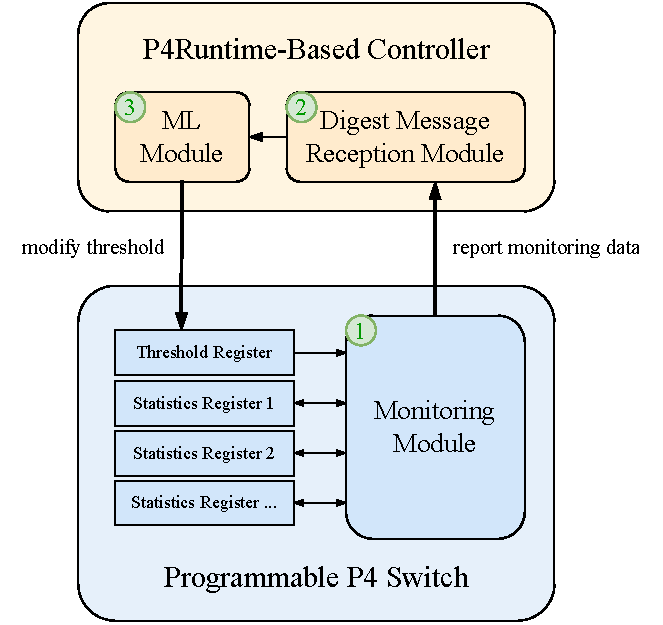
\includegraphics[width=0.45\textwidth]{./figures/arch.pdf}
    \caption{MAT4PM Architecture.}
    \label{arch}
\end{figure}

Figure~\ref{arch} illustrates the overall architecture of the MAT4PM system. 
The framework consists of three functional modules distributed across the data plane and the control plane, which collaborate to deliver efficient and intelligent traffic monitoring. 
The module numbers below correspond to those in the figure:

\begin{enumerate}
    \item \textbf{Monitoring Module}: Deployed on programmable P4 switches, this data plane component collects real-time traffic statistics and triggers reports when any monitored metric exceeds a predefined threshold.
    \item \textbf{Digest Message Reception Module}: Located on the controller based on P4Runtime~\cite{P4Runtime}, this module receives and processes statistical reports from switches and invokes the ML Module.
    \item \textbf{ML Module}: Responsible for inferring the optimal monitoring threshold based on the current traffic conditions and issuing the updated threshold to the switch for the next monitoring cycle.
\end{enumerate}

% These modules operate in a closed-loop workflow, where data plane events drive control plane decisions, and updated decisions are fed back to the data plane for continuous adaptation. 
\rev{These modules form a closed-loop workflow: data plane events trigger control plane decisions, which are then fed back to the data plane for continuous adaptation.} 
During system operation, the P4 switch continuously collects traffic statistics from passing packets, such as the number of packets and bytes within a fixed window. 
Simultaneously, it maintains a set of registers that store the current monitoring thresholds. 
These registers are used to determine whether an update should be triggered based on real-time traffic. 
When any monitored metric (e.g., packet or byte count within a window, or the elapsed time since the last report) exceeds its corresponding threshold, the switch immediately initiates a proactive reporting mechanism, sending a digest message containing the relevant statistics to the controller. 
Upon each reporting event, local counters are reset, initiating a new monitoring cycle and ensuring an event-driven, low-latency response mechanism.

Upon receiving digest messages from the switch, the controller first parses the report and extracts the traffic-related features. 
It then invokes a pre-trained machine learning model to predict the optimal threshold for the current network state. 
This prediction considers both monitoring accuracy and communication cost, striking a dynamic balance between precision and overhead. 
The newly predicted threshold is then written back into the relevant switch registers, allowing subsequent monitoring actions to proceed under updated conditions.

In subsequent algorithmic descriptions, experimental setups, and performance evaluations, we use the monitoring period threshold $prd_m$ as a representative example for triggering reporting actions. 
Specifically, during each monitoring interval, the system checks whether the time since the last report for a given flow exceeds its designated $prd_m$ threshold. 
If so, a new report is triggered. 
This time-based triggering mechanism is both simple and generalizable, making it suitable for various scenarios. 
Regarding the selected monitoring features, this work focuses on two fundamental yet critical traffic indicators: packets per second (pps) and bits per second (bps). 
These metrics are widely adopted in network performance analysis and anomaly detection, as they effectively capture dynamic traffic behaviors and provide highly relevant input features for subsequent error evaluation and threshold optimization.

To validate the feasibility of the proposed method and conduct functional testing, the system is implemented on BMv2 (Behavioral Model version 2)~\cite{BMv2}, the official open-source software switch for P4. 
\rev{
It is important to note that BMv2 primarily serves as a development and debugging platform and does not incorporate performance-oriented optimizations typically found in production-grade switching systems. 
Compared to optimized software switches such as Open vSwitch (OVS)~\cite{OVS}, as well as hardware-based programmable switching platforms including Tofino ASIC~\cite{TFTG}, BMv2 exhibits substantially lower packet processing throughput and higher per-packet processing latency. 
This performance gap arises from the interpretive execution model and lack of hardware acceleration in BMv2, which distinguishes it from both high-performance software data planes and specialized programmable hardware. 
Accordingly, the experimental evaluation in this study emphasizes functional correctness and feasibility analysis of the proposed mechanisms, rather than throughput-oriented benchmarking or performance comparison under line-rate deployment conditions.
}

\subsubsection{Monitoring Threshold Configuration and Retrieval}

Algorithm~\ref{algo_thld} illustrates how the MAT4PM system stores and retrieves the monitoring period threshold $prd_m$. 
Since the P4 language does not support the direct definition or access of global variables, the system employs registers to preserve state across packets. 
This design enables each monitored flow to independently maintain its current threshold configuration, adhering to the constraints of the P4 language while supporting efficient per-flow indexing and updates via flow identifiers.

Specifically, the system defines a register array named $prds_m$ to store the reporting period thresholds for all monitored flows, where each entry corresponds to a specific flow. 
Let $N_{flow}$ denote the total number of monitored flows, and the register must support indexable access to up to $N_{flow}$ distinct entries. 
To ensure correct address computation, the index width is set at compile time to $\lceil \log_2 N_{flow} \rceil$, guaranteeing a unique mapping for each flow identifier within the supported range. 
This mechanism ensures that each flow has an independent and dynamically adjustable monitoring period, which is a critical component enabling MAT4PM's fine-grained adaptive monitoring capabilities.

\begin{algorithm}[!t]
    \caption{Monitoring threshold configuration and retrieval}
    \label{algo_thld}
    \begin{algorithmic}[1]
        \STATE // The \textbf{register} below is used to store the monitoring period thresholds.
        \STATE \textbf{register}$<$bit$<$48$>$, bit$<\lceil \log_2 N_{flow} \rceil>>$($N_{flow}$) $prds_m$;
        \STATE
        \STATE // The \textbf{function} below retrieves the monitoring period threshold.
        \STATE bit$<$48$>$ get\_thld(in bit$<\lceil \log_2 N_{flow} \rceil> flow\_num$) \{
        \STATE \hspace{1em} bit$<$48$>$ $prd_m$;
        \STATE \hspace{1em} $prds_m$.read($prd_m$, $flow\_num$);
        \STATE \hspace{1em} return $prd_m$;
        \STATE \}
    \end{algorithmic}
\end{algorithm}

\subsubsection{Monitoring Data Report}

In programmable P4 switches, there are typically two mechanisms for transmitting data plane information to the control plane: the packet-in mechanism, where a complete packet carrying the required information is encapsulated and sent to the controller; and the digest mechanism, which transmits only selected structured fields in the form of a lightweight message. 
% In the MAT4PM system, the digest mechanism is adopted for reporting monitoring results from the data plane, based on comprehensive considerations of performance and communication efficiency which are illustrated as follows.
\rev{In the MAT4PM system, the digest mechanism is adopted for reporting monitoring results from the data plane, due to its advantages in performance and communication efficiency, as discussed below.}

The packet-in approach generally forwards the entire packet, including the header and payload, as a distinct stream message under P4Runtime. 
Although this method offers flexibility, it incurs high communication overhead, especially in network monitoring scenarios where frequent reporting is required. 
Such frequent transmissions significantly burden bandwidth and control channels. 
Moreover, each packet-in message is triggered as an independent event, limiting opportunities for aggregation and batching, and consequently affecting scalability under high-volume reporting. 
In contrast, the digest mechanism allows switches to transmit only essential monitoring fields, such as statistical counters or metadata, without carrying full packet content, thereby substantially reducing message size. 
Additionally, multiple digest messages can be automatically aggregated by the P4Runtime server at the switch side and forwarded to the controller in batch mode. 
This batching capability notably improves transmission efficiency. 
More importantly, digest functions can only be invoked in the ingress control path, aligning seamlessly with MAT4PM's monitoring logic, which is also deployed in the ingress stage. 
Considering all these factors, the digest mechanism represents the optimal strategy for implementing event-driven reporting in MAT4PM.

Algorithm~\ref{algo_report} describes the procedure through which MAT4PM uses digest messages to report monitoring data. 
Each digest encapsulates the unique identifier of the monitored flow ($flow\_num$) along with its associated metrics, including the total number of bytes and packets, as well as the elapsed time since the last report.

\begin{algorithm}[!t]
    \caption{Monitoring data report}
    \label{algo_report}
    \begin{algorithmic}[1]
        \STATE // The \textbf{registers} below are used to store monitoring data.
        \STATE \textbf{register}$<$bit$<$32$>$, bit$<\lceil \log_2 N_{flow} \rceil>>$($N_{flow}$) $pkts$;
        \STATE \textbf{register}$<$bit$<$32$>$, bit$<\lceil \log_2 N_{flow} \rceil>>$($N_{flow}$) $bytes$;
        \STATE \textbf{register}$<$bit$<$48$>$, bit$<\lceil \log_2 N_{flow} \rceil>>$($N_{flow}$) $times$;
        \STATE
        \STATE // Digest Message Struct.
        \STATE \textbf{struct} reported\_data \{
        \STATE \hspace{1em} bit$<\lceil \log_2 N_{flow} \rceil>$ flow\_num;
        \STATE \hspace{1em} bit$<$48$>$ timestamp\_delta;
        \STATE \hspace{1em} bit$<$32$>$ reported\_pkt;
        \STATE \hspace{1em} bit$<$32$>$ reported\_byte;
        \STATE \}
        \STATE
        \STATE // The \textbf{function} below is used to send digest message.
        \STATE void report\_to\_controller(
        \STATE \hspace{1em} in bit$<\lceil \log_2 N_{flow} \rceil>$ $flow\_num$,
        \STATE \hspace{1em} in bit$<$48$>$ $timestamp\_delta$
        \STATE ) \{
        \STATE \hspace{1em} reported\_data data;
        \STATE \hspace{1em} data.flow\_num = flow\_num;
        \STATE \hspace{1em} data.timestamp\_delta = timestamp\_delta;
        \STATE \hspace{1em} $pkts$.read(data.reported\_pkt, $flow\_num$);
        \STATE \hspace{1em} $bytes$.read(data.reported\_byte, $flow\_num$);
        \STATE \hspace{1em} digest$<$reported\_data$>$(1, data);
        \STATE \}
    \end{algorithmic}
\end{algorithm}

\subsubsection{Data Plane Monitoring Mechanism}

Figure~\ref{ingress} illustrates the internal processing workflow for traffic monitoring within the packet processing pipeline of a programmable P4 switch. 
The monitoring logic is primarily implemented in the ingress control block and comprises two critical actions: one responsible for flow monitoring (denoted as the Monitoring Action) and the other for triggering the reporting mechanism (denoted as the Reporting Action). 
Together, these ensure real-time statistics updates and event-driven monitoring data reporting.

\begin{figure}[!t]
    \centering
    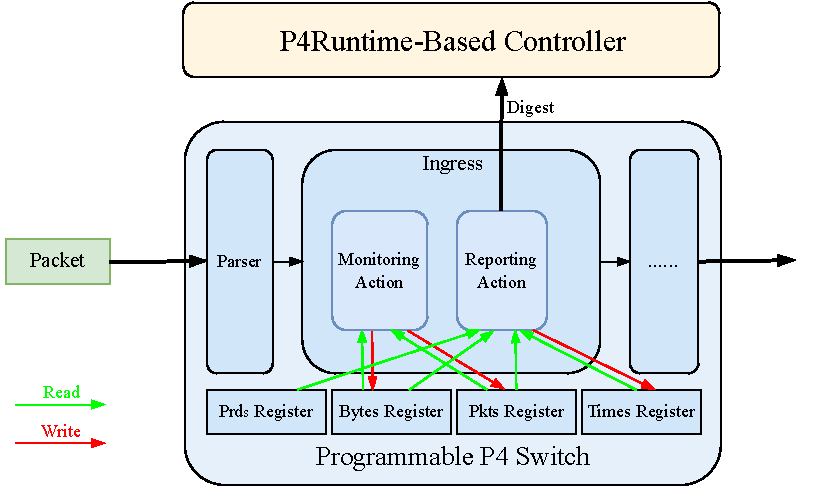
\includegraphics[width=0.5\textwidth]{./figures/ingress.pdf}
    \caption{Processing pipeline in data planes.}
    \label{ingress}
\end{figure}

Upon arrival at the switch, a packet is first parsed by the P4 parser, which extracts header fields layer by layer. 
The packet then proceeds to the ingress match-action stage, where it is matched against flow table entries. 
If a match is found, the system executes the monitoring action. 
This action uses the flow identifier as an index to access two monitoring registers: $bytes$ and $pkts$, which accumulate the total number of bytes and packets received for the corresponding flow, respectively. 
After incrementing these values based on the current packet, the updated counters are written back to the registers, enabling per-packet granularity in flow statistics collection.

Following the update of monitoring registers, the packet processing enters the reporting action. 
At this stage, the system reads the last report timestamp for the current flow from the $times$ register. 
It then calculates the time elapsed since the last report using the current system timestamp, which is obtained from the standard ingress metadata (\texttt{standard\_metadata.ingress\_global\_timestamp}). 
The reporting threshold for this flow, denoted as $prd_m$, is retrieved from the $prds$ register. 
If the elapsed time exceeds or equals $prd_m$, the reporting condition is satisfied, and a digest message is immediately generated to send the current flow statistics to the controller. 
Simultaneously, the monitoring counters in $bytes$ and $pkts$ are reset to zero to begin a new monitoring interval, and the current timestamp is written back to $times$ as a reference for the next report cycle.

This monitoring and reporting mechanism relies heavily on stateful registers and an event-driven design, enabling responsive data plane monitoring with minimal latency. 
It fully leverages the programmability of P4 and provides a high-quality data foundation for the controller's subsequent machine learning-based threshold adaptation. 
The corresponding P4 pseudocode implementation is presented in Algorithm~\ref{algo_ingress}.

\begin{algorithm}[!t]
    \caption{Data plane monitoring mechanism}
    \label{algo_ingress}
    \begin{algorithmic}[1]
        \STATE \textbf{control} Ingress(inout headers hdr,
        \STATE \hspace{1em} inout metadata meta,
        \STATE \hspace{1em} inout standard\_metadata\_t standard\_metadata) \{
        \STATE \hspace{1em} // The \textbf{action} below is the monitoring operation for flows.
        \STATE \hspace{1em} \textbf{action} monitor\_flow(in bit$<\lceil \log_2 N_{flow} \rceil>$ $flow\_num$) \{
        \STATE \hspace{2em} bit$<$32$>$ pkt, byte;
        \STATE \hspace{2em} $pkts$.read(pkt, $flow\_num$);
        \STATE \hspace{2em} $bytes$.read(byte, $flow\_num$);
        \STATE \hspace{2em} pkt = pkt + 1;
        \STATE \hspace{2em} byte = byte + standard\_metadata.packet\_length;
        \STATE \hspace{2em} $pkts$.write($flow\_num$, pkt);
        \STATE \hspace{2em} $bytes$.write($flow\_num$, byte);
        \STATE \hspace{1em} \}
        \STATE \hspace{1em} // The {\bf action} below determines whether to report the monitoring data based on the monitoring threshold.
        \STATE \hspace{1em} {\bf action} report\_flow(in bit$<\lceil \log_2 N_{flow} \rceil>$ $flow\_num$) \{
        \STATE \hspace{2em} bit$<$48$>$ time, now, delta;
        \STATE \hspace{2em} $times$.read(time, $flow\_num$);
        \STATE \hspace{2em} now = standard\_metadata.ingress\_global\_timestamp;
        \STATE \hspace{2em} delta = now - time;
        \STATE \hspace{2em} // Function get\_thld() is implemented in Algorithm~\ref{algo_thld}.
        \STATE \hspace{2em} \textbf{if} (delta $>=$ get\_thld($flow\_num$)) \{
        \STATE \hspace{3em} // The implementation of report\_to\_controller() is presented in Algorithm~\ref{algo_report}.
        \STATE \hspace{3em} report\_to\_controller($flow\_num$, delta);
        \STATE \hspace{3em} // Reset the monitoring data of this flow.
        \STATE \hspace{3em} $pkts$.write($flow\_num$, 0);
        \STATE \hspace{3em} $bytes$.write($flow\_num$, 0);
        \STATE \hspace{3em} // Update the last reported time of this flow.
        \STATE \hspace{3em} $times$.write($flow\_num$, now);
        \STATE \}\}\}
    \end{algorithmic}
\end{algorithm}

\subsubsection{Control Plane Decision Processing Mechanism}

Figure~\ref{controller} illustrates the core internal processing workflow of the MAT4PM controller. 
Within the system architecture, the \textit{Digest Message Reception Module} is responsible for receiving and handling digest messages transmitted from the data plane. 
Upon receiving a new report, this module parses the message and extracts essential monitoring features, including the flow identifier, the number of packets, the total byte count, and the elapsed time since the last report. 
% These extracted features are then assembled into a standardized input vector and passed to a pre-trained machine learning model for inference, which outputs the optimal monitoring interval threshold for the given flow. 
\rev{These extracted features are assembled into a standardized input vector and passed to a pre-trained machine learning model for inference. The model outputs the optimal monitoring interval threshold for the given flow.} 
Once the predicted threshold is obtained, the controller proceeds to synchronize this value with the data plane to update the local monitoring policy at the switch level.

\rev{To mitigate unnecessary consumption of control plane bandwidth caused by frequent minor updates that contribute little to monitoring effectiveness}, MAT4PM integrates a threshold update suppression mechanism. 
Specifically, the controller maintains a local hash table \rev{to store the most recently enforced monitoring thresholds for all active flows}. 
When a new threshold is predicted, \rev{it is compared against the previously applied value associated with the same flow}. 
\rev{A control plane update is triggered only if the relative difference between the two exceeds a configurable suppression margin (e.g., 10\%). 
This margin is a tunable system parameter that can be adjusted according to deployment requirements, traffic dynamics, and control plane resource constraints, rather than a fixed constant embedded in the design.}

\rev{
If the suppression condition is satisfied, a \texttt{write\_register} instruction is issued to update the monitoring threshold stored in the corresponding switch register. 
Otherwise, the update is deferred, allowing the data plane to continue operating under the existing configuration. 
By filtering out insignificant threshold variations caused by short-term traffic fluctuations or minor prediction noise, this mechanism reduces control plane communication overhead and improves system stability, while preserving the ability to react to meaningful traffic changes. 
The complete control logic, encompassing digest message reception, feature extraction, machine learning-based inference, and conditional threshold updates, is summarized in Algorithm~\ref{algo_controller}.
}

\begin{figure}[!t]
    \centering
    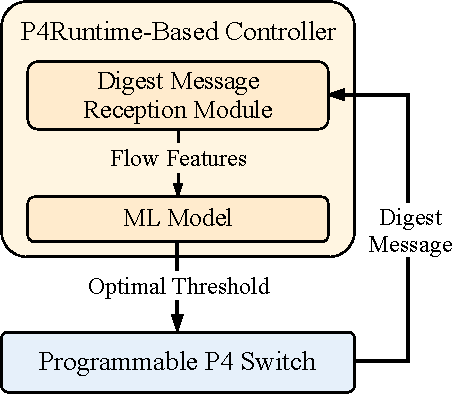
\includegraphics[width=0.32\textwidth]{./figures/controller.pdf}
    \caption{Internal processing workflow of a controller.}
    \label{controller}
\end{figure}

\begin{algorithm}[!t]
    \caption{Control plane decision processing mechanism}
    \label{algo_controller}
    \begin{algorithmic}[1]
        \WHILE{true}
        \STATE // Wait and receive digest messages.
        \STATE $msg$ $\Leftarrow$ \texttt{get\_digest\_message()};
        \STATE // Parse $msg$ to extract the monitoring data.
        \STATE $flow\_num,\ \Delta t,\ packets,\ bytes \Leftarrow msg$.\texttt{parse()};
        \STATE $pps,\ bps \Leftarrow packets / \Delta t,\ (bytes \times 8) / \Delta t;$
        \STATE // Construct feature vector $\mathbf{x}$.
        \STATE $\mathbf{x} \Leftarrow \{bps,\ pps\}$;
        \STATE // Predict optimal threshold.
        \STATE $prd_m^* \Leftarrow \texttt{ML\_Model.Predict}(\mathbf{x})$;
        \IF{$\lvert ( prd_m^* - old\_prd_m ) / old\_prd_m \rvert > 10\%$}
        \STATE // Update the threshold for this flow.
        \STATE \texttt{write\_register($flow\_num$, $prd_m^*$)};
        \ENDIF
        \ENDWHILE
    \end{algorithmic}
\end{algorithm}

\subsection{Optimal Threshold Definition}
\label{subsection32}

\noindent To construct a labeled dataset suitable for training a machine learning model, it is first necessary to rigorously define the concept of an optimal monitoring period threshold. 
This section derives the definition starting from basic traffic rate metrics, followed by error modeling, communication cost estimation, and finally the formulation of a composite cost function for determining the optimal threshold.

Two fundamental traffic rate indicators are considered: bit rate (bps, bits per second) and packet rate (pps, packets per second). 
For traffic observed over a continuous time window, the rates are defined as:
\begin{equation}
    bps = \frac{\text{Total Bytes} \times 8}{\Delta t} ,
\end{equation}
\begin{equation}
    pps = \frac{\text{Total Packets}}{\Delta t} ,
\end{equation}
where $\Delta t$ denotes the duration of the observation interval in seconds, while Total Bytes and Total Packets refer to the number of bytes and packets recorded during this interval, respectively. 
In practice, the reported rate by the switch may deviate from the ground-truth rate derived via offline analysis. 
To quantify such deviations, two separate relative error metrics are defined:

\begin{equation}
    \label{eq:err_bps}
    E_{bps} = \left| \frac{bps_{reported} - bps_{true}}{bps_{true}} \right| ,
\end{equation}

\begin{equation}
    \label{eq:err_pps}
    E_{pps} = \left| \frac{pps_{reported} - pps_{true}}{pps_{true}} \right| ,
\end{equation}
where $bps_{reported}$ and $pps_{reported}$ denote the bit rate and packet rate reported by the switch, while $bps_{true}$ and $pps_{true}$ are their respective ground-truth values obtained from packet trace analysis. 
A simple linear combination is used to define the overall monitoring error:

\begin{equation}
    \label{eq:E}
    E = E_{bps} + E_{pps} .
\end{equation}

The monitoring threshold $prd_m$ (in milliseconds) not only affects the accuracy of measurements but also directly influences the communication overhead between the data and control planes. 
Smaller thresholds lead to more frequent reporting, increasing control channel load. 
The reporting frequency per unit time is thus defined as:
\begin{equation}
    \label{eq:C}
    C = \frac{1}{prd_m} .
\end{equation}
To integrate $C$ with $E$ in a unified optimization framework, normalization is required. 
A maximum reporting frequency $C_{max} = 50$ is adopted as the normalization constant, implying that up to 50 monitoring reports per second are permitted per switch. 
This upper bound is based on practical engineering observations regarding the capacity of SDN controllers and the tolerance of control plane bandwidth. 
Exceeding this threshold has been shown to cause undesirable effects such as increased controller CPU load, control message queuing, packet loss, and latency. 
Therefore, $C_{max} = 50$ reflects a realistic limit for maintaining system responsiveness without overburdening the control infrastructure. 
The normalized communication cost is computed as:
\begin{equation}
    \label{eq:Cnorm}
    C_{norm} = \frac{C}{C_{max}} ,
\end{equation}
ensuring that $C_{norm} \in [0, 1]$, which enables consistent weighting with the monitoring error term.

The overall cost of a monitoring strategy is then formulated as:
\begin{equation}
    \label{eq:cost(prd_m)}
    cost(prd_m) = \alpha \cdot E + \beta \cdot C_{norm}, \quad \alpha + \beta = 1 ,
\end{equation}
where $\alpha$ and $\beta$ are tunable hyperparameters that control the trade-off between monitoring accuracy and communication overhead. 
In subsequent experiments, $\alpha = 0.6$ and $\beta = 0.4$ are used, slightly favoring accuracy over overhead reduction.

The optimal monitoring threshold $prd_m^*$ is defined as the value that minimizes the overall cost for a given traffic sample. 
An exhaustive search method is employed to evaluate all candidate thresholds within a predefined interval of $[20, 1500]$ milliseconds, covering the practical range from high-frequency to low-frequency monitoring. 
The optimal threshold is formally expressed as:
\begin{equation}
    prd_m^* = \arg\min_{prd_m \in [20, 1500]} cost(prd_m) .
\end{equation}
This definition enables the labeling of each flow sample with its corresponding optimal monitoring period, thereby facilitating the construction of a high-quality supervised learning dataset essential for subsequent model training.

\subsection{Data Processing}
\label{subsection33}

\noindent
% To construct a high-quality labeled dataset suitable for training machine learning models, this section provides a detailed description of the data acquisition, processing, and labeling workflow.
\rev{This subsection describes the data acquisition, processing, and labeling workflow used to construct the training dataset.}

During the initialization of the BMv2 software switch using the \texttt{simple\_switch\_grpc} command, the \texttt{--pcap} parameter is configured to specify the output directory for packet capture (PCAP) files. 
This setting enables the switch to record all transiting packets during runtime into standardized PCAP format files. 
PCAP is a widely adopted data interchange format in network analysis, extensively used in diagnostics, security auditing, and performance evaluation. 
It preserves complete packet-level information, including protocol headers, payloads, timestamps, and packet lengths. 
Due to its broad compatibility, PCAP data can be parsed and analyzed using mainstream tools such as Wireshark, Tshark, and Tcpreplay, making it suitable for offline traffic reconstruction and anomaly detection research.

Once a traffic batch is generated, the corresponding PCAP file is extracted as the ground-truth reference. 
For an accurate replay that aligns with the original capture rate, packet playback is conducted using Scapy, which enables fine-grained control over the transmission interval of individual packets. 
Unlike tools such as Tcpreplay, which transmits packets as fast as possible, or playcap, which is primarily designed for loopback testing scenarios, Scapy allows for precise timing replication of the original traffic. 
This ensures that the replayed packet stream closely matches the temporal dynamics of the original capture, thereby preserving the fidelity of flow rates within each monitoring window.

Under the premise of accurately replayed traffic, the system then performs multiple experimental cycles under varying monitoring thresholds $prd_m$, ensuring that each configuration is evaluated under identical traffic conditions. 
For a given threshold, the number of bytes and packets in each reporting window is extracted from the PCAP file to compute the true bit rate and packet rate. 
These values are then compared against the switch-reported metrics to compute the monitoring error using the previously defined error functions. Subsequently, the communication cost and the total cost are computed using the normalized formulas introduced earlier.

For each fixed traffic rate, multiple candidate thresholds are evaluated. 
The corresponding total costs are recorded, and the threshold that minimizes the cost function is selected as the optimal monitoring threshold $prd_m^*$ for that traffic condition. The system then transitions to a new traffic configuration and repeats the same procedure until the entire range of predefined traffic conditions is covered.

The resulting dataset consists of three attributes: the reported bit rate (\texttt{reported\_bps}), the reported packet rate (\texttt{reported\_pps}), and the corresponding optimal monitoring threshold (\texttt{optimal\_prdm}). 
These two reported metrics are selected as input features because, in practical deployment scenarios, the switch can only provide flow statistics it measures directly. 
True rates (such as \texttt{true\_bps} and \texttt{true\_pps}) are only available during offline dataset construction and cannot be accessed during real-time operation. 
Hence, the model training process strictly emulates real-world conditions by using only observable switch-reported data, ensuring the deployability and operational feasibility of the trained model.

Through this rigorous data processing and labeling pipeline, a diverse and well-annotated dataset is constructed, spanning a wide range of traffic conditions and embedding optimal threshold labels. 
This provides a solid foundation for training and evaluating machine learning models in subsequent sections. The overall process is summarized in Algorithm~\ref{algo_collection}.

\begin{algorithm}[!t]
    \caption{Data processing}
    \label{algo_collection}
    \begin{algorithmic}[1]
        \STATE \textbf{Initialize:} candidate thresholds $prds_m = [20, 1500]$ ms
        \FOR{each traffic rate setting}
        \STATE Start BMv2 with PCAP recording enabled.
        \STATE Replay captured packets at original timing using Scapy.
        \FOR{each threshold $prd_m$ \textbf{in} $prds_m$}
        \STATE Set $prd_m$ as the current monitoring threshold.
        \STATE Monitor and record reported \texttt{bps}, \texttt{pps} during replay.
        \STATE Compute real \texttt{bps} and \texttt{pps} from PCAP ground truth.
        \STATE Calculate error metric $E$ according to Eq.~\ref{eq:E}.
        \STATE Calculate communication cost $C$ according to Eq.~\ref{eq:Cnorm}.
        \STATE Evaluate total cost $cost(prd_m)$ according to Eq.~\ref{eq:cost(prd_m)}.
        \ENDFOR
        \STATE Find $prd_m^* = \arg\min cost(prd_m)$ over all candidates.
        \STATE Store sample: $\{\texttt{reported\_bps}, \texttt{reported\_pps}\} \rightarrow prd_m^*$.
        \ENDFOR
    \end{algorithmic}
\end{algorithm}

\section{Experiments and Evaluation}
\label{sec4}

\subsection{Experimental Setup}

\noindent This subsection outlines the experimental environment and software configurations adopted to ensure methodological rigor and reproducibility of the results. 
All experiments were conducted within a virtualized environment deployed on a single physical host. 
The virtualization platform used was VirtualBox version 5.2.42, running a 64-bit Ubuntu 24.10 virtual machine instance. 
The virtual machine was allocated 4 GB of memory and operated on an Intel i5-13500H CPU. 
The Python environment version 3.12.3 was employed to support tasks including network emulation, data processing, control plane implementation, and machine learning model training and inference.

For network emulation, Mininet 2.3.1~\cite{Mininet} was utilized to construct the network topology and manage traffic scheduling. 
The data plane was implemented using the BMv2 software switch. 
P4 programs were developed following the P4\textsubscript{16} language specification and compiled with the p4c compiler version 1.2.4.15, targeting the official V1Model 20200408 architecture. 
The control plane was realized using P4Runtime version 1.3.0, facilitating flow table configuration, register access, and message handling. 
Traffic generation was handled by iPerf 2.1.9~\cite{iPerf}, which produced consistent TCP/UDP traffic. 
In addition, Scapy version 2.5.0~\cite{SCAPY} was employed to parse PCAP files and replay traffic, allowing fine-grained control over packet rates and inter-packet intervals during data collection.

\rev{
It is worth noting that alternative software switches such as OVS are not used for experimental comparison in this study. 
Although OVS is widely deployed in virtualized environments, it does not natively support the P4 programming model, nor does it provide mechanisms equivalent to P4 registers, digest messages, or in-switch stateful processing required for event-driven monitoring and proactive reporting. 
Similarly, performance-optimized variants such as OVS with DPDK (Data Plane Development Kit)~\cite{DPDK} primarily focus on accelerating packet I/O throughput, but still lack native support for P4-based programmable pipelines and control plane driven asynchronous telemetry primitives. 
As a result, a direct comparison between BMv2 and OVS or OVS with DPDK would be methodologically inappropriate for evaluating the functional correctness and adaptive behavior of P4-based monitoring mechanisms.
}

The experimental topology is illustrated in Figure~\ref{topo}, consisting of two BMv2 software switches and two host nodes, with each switch connected to one host. 
The switches were directly interconnected and linked to a centralized controller. 
A total of 100 flows were configured during the experiments, leading to a P4 register index width of 7 bits ($\lceil \log_2 100 \rceil$).

\begin{table*}[!t]
    \centering
    \caption{Summary of experimental environment and software configurations.}
    \label{env_table}
    \begin{tabular}{p{0.32\textwidth} p{0.48\textwidth}<{\raggedright}}
        \toprule
        \textbf{Category} & \textbf{Configuration Details} \\
        \midrule
        \textbf{Host Hardware} & Intel i5-13500H CPU, 4 GB RAM \\
        \textbf{Virtualization} & VirtualBox 5.2.42, Ubuntu 24.10 (64-bit VM) \\
        \textbf{Python Environment} & Python 3.12.3 \\
        \textbf{Network Emulation} & Mininet 2.3.1, BMv2 switch \\
        \textbf{P4 Compilation} & P4\textsubscript{16}, V1Model 20200408, p4c 1.2.4.15 \\
        \textbf{Control Plane} & P4Runtime 1.3.0 \\
        \textbf{Traffic Generation} & iPerf 2.1.9, Scapy 2.5.0 \\
        \textbf{ML Frameworks} & scikit-learn 1.5.2 (SVM), LightGBM 4.6.0, XGBoost 1.7.6 \\
        \textbf{Hyperparameter Tuning} & Optuna 4.2.1 \\
        \textbf{Configured Flow Count} & 100 flows; register index width = 7 bits \\
        \bottomrule
    \end{tabular}
\end{table*}

To facilitate quick reference to the experimental setup, Table~\ref{env_table} summarizes the hardware specifications, virtualization settings, network emulation tools, and machine learning frameworks used throughout the evaluation. 
The selection and configuration of these components were designed to ensure that the results are both reproducible and representative of realistic deployment conditions.

\begin{figure}[!t]
    \centering
    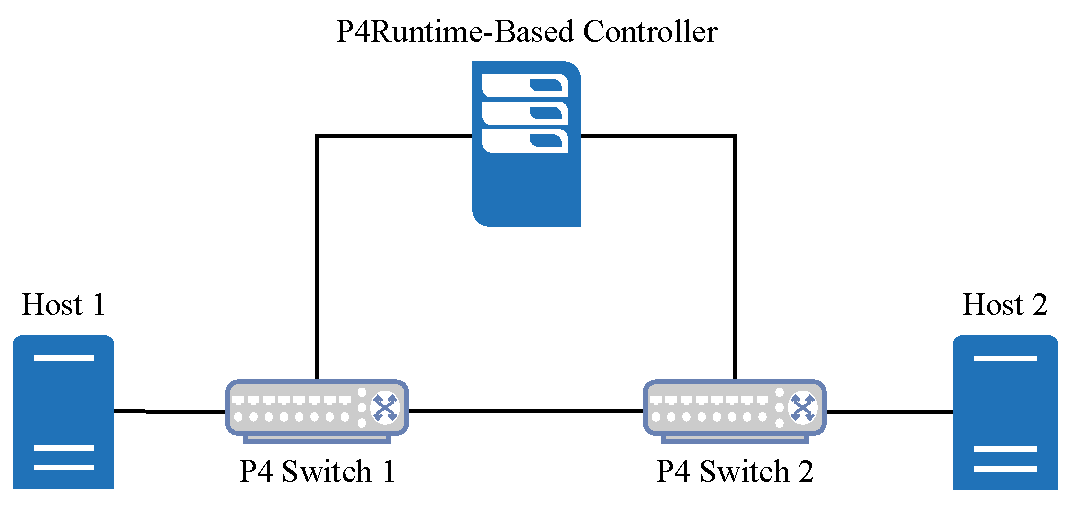
\includegraphics[width=0.48\textwidth]{./figures/topo.pdf}
    \caption{Network topology.}
    \label{topo}
\end{figure}

The training and hyperparameter optimization of machine learning models relied on the following software packages: scikit-learn 1.5.2~\cite{Scikit-learn} was used to construct and evaluate the SVM models; LightGBM 4.6.0 and XGBoost 1.7.6 were employed to implement lightweight and high-efficiency gradient boosting frameworks, respectively. 
Hyperparameter tuning was conducted using Optuna version 4.2.1~\cite{Optuna}, enabling automated search strategies to enhance model performance.

\rev{
To further support transparency and reproducibility, the complete source code, experimental scripts, and configuration files used in this study are publicly available in an open-access repository~\cite{MAT4PM}. 
The repository includes the P4 data plane programs, controller-side implementation code, machine learning training and inference code, as well as Mininet topology scripts and traffic generation configurations. 
All experiments reported in this paper can be reproduced under the specified software environment detailed in this subsection.
}

\subsection{Model Training Details}
\label{subsection42}

\noindent
% To comprehensively evaluate the adaptive threshold inference capabilities of the MAT4PM system across different learners, three mainstream regression models---XGBoost, LightGBM, and SVM---are trained using the labeled dataset collected in the experiments. 
\rev{Three mainstream regression models, namely XGBoost, LightGBM, and SVM, are trained on the labeled dataset to evaluate the adaptive threshold inference capability of MAT4PM.} 
XGBoost is a widely adopted ensemble learning algorithm based on gradient boosted decision trees, known for its high predictive accuracy and scalability. 
LightGBM is a histogram-based boosting framework designed for fast training and low memory usage, particularly suitable for real-time applications. 
% SVM is effective for capturing nonlinear relationships through kernel-based learning, offering strong generalization even with limited training data. 
\rev{SVM captures nonlinear relationships through kernel-based learning and maintains robust generalization with limited training data.} 
All models are developed using supervised learning, with the reported byte rate (\texttt{reported\_bps}) and packet rate (\texttt{reported\_pps}) as input features, and the optimal monitoring threshold (\texttt{optimal\_prdm}) as the regression target. 
The dataset is randomly split into training and validation sets at an 8:2 ratio. 
The training set is used for model fitting, while the validation set is utilized for hyperparameter tuning and performance evaluation.

To enhance model performance and reduce manual tuning bias, Bayesian optimization is applied for automated hyperparameter selection. 
Each model is trained over 100 trials (\texttt{n\_trials} = 100) within a predefined search space, with mean squared error (MSE) on the validation set serving as the evaluation metric. 
The final configurations obtained through Bayesian optimization are summarized in Table~\ref{tab:hyperparams}, which presents key hyperparameter settings for each model. 
This tabular presentation facilitates a clear comparison of tuning results across model types, supporting reproducibility and implementation transparency.

\begin{table}[!t]
    \centering
    \caption{Optimal hyperparameter configurations for each machine learning model.\label{tab:hyperparams}}
    \begin{tabular}{p{0.14\textwidth} p{0.18\textwidth} p{0.06\textwidth}<{\centering}}
        \toprule
        \textbf{Model} & \textbf{Hyperparameter} & \textbf{Value} \\
        \midrule
        \multirow{8}{*}{\textbf{XGBoost}} 
        & \texttt{n\_estimators} & 359 \\
        & \texttt{learning\_rate} & 0.0134 \\
        & \texttt{max\_depth} & 3 \\
        & \texttt{gamma} & 0.2812 \\
        & \texttt{subsample} & 0.6055 \\
        & \texttt{colsample\_bytree} & 0.7713 \\
        & \texttt{reg\_alpha} & 0.0077 \\
        & \texttt{reg\_lambda} & 0.3537 \\
        \midrule
        \multirow{7}{*}{\textbf{LightGBM}} 
        & \texttt{num\_leaves} & 31 \\
        & \texttt{learning\_rate} & 0.1301 \\
        & \texttt{feature\_fraction} & 0.7988 \\
        & \texttt{bagging\_fraction} & 0.8462 \\
        & \texttt{min\_data\_in\_leaf} & 36 \\
        & \texttt{reg\_alpha} & 0.3431 \\
        & \texttt{reg\_lambda} & 0.0394 \\
        \midrule
        \multirow{4}{*}{\textbf{SVM (Sigmoid)}} 
        & \texttt{C} & 152.5498 \\
        & \texttt{epsilon} & 0.8845 \\
        & \texttt{gamma} & 0.0192 \\
        & \texttt{degree} & 4 \\
        \bottomrule
    \end{tabular}
\end{table}

To assess the deployability of each model in real-world systems, memory consumption and prediction latency are measured. 
Upon loading, the memory footprint of each model is recorded as follows: XGBoost—30.99 KB, LightGBM—13.89 KB, and SVM—36.24 KB. 
These values indicate that all models exhibit minimal memory overhead, rendering them suitable for deployment on resource-constrained switches, controllers, or edge nodes.

Inference efficiency is further evaluated using the Python \texttt{timeit} module. 
Each model performs 1000 consecutive predictions after loading, and the execution time for each inference is recorded. 
The distribution of individual prediction times is illustrated in Figure~\ref{PredictionTimeCostsLine}. 
% The results show that the majority of predictions are completed within 1~ms, with only occasional outliers. 
\rev{Most predictions are completed within 1~ms, with only occasional outliers.} 
Specifically, XGBoost, LightGBM, and SVM achieve maximum prediction latencies of 4.545~ms, 3.920~ms, and 2.282~ms respectively, all significantly under the 5~ms soft real-time threshold empirically defined for this application scenario.

To better visualize the central tendency and variance in prediction latency, boxplots are generated for all models, as shown in Figure~\ref{PredictionTimeCostsBox}. 
Outliers are excluded based on default settings, and the mean inference time is marked by green triangles. 
The average prediction time is 0.949~ms for XGBoost, 0.771~ms for LightGBM, and 0.789~ms for SVM. 
These results confirm the suitability of all three models for real-time inference in MAT4PM, meeting the latency requirements of dynamic SDN monitoring scenarios.

\begin{figure}[!t]
    \centering
    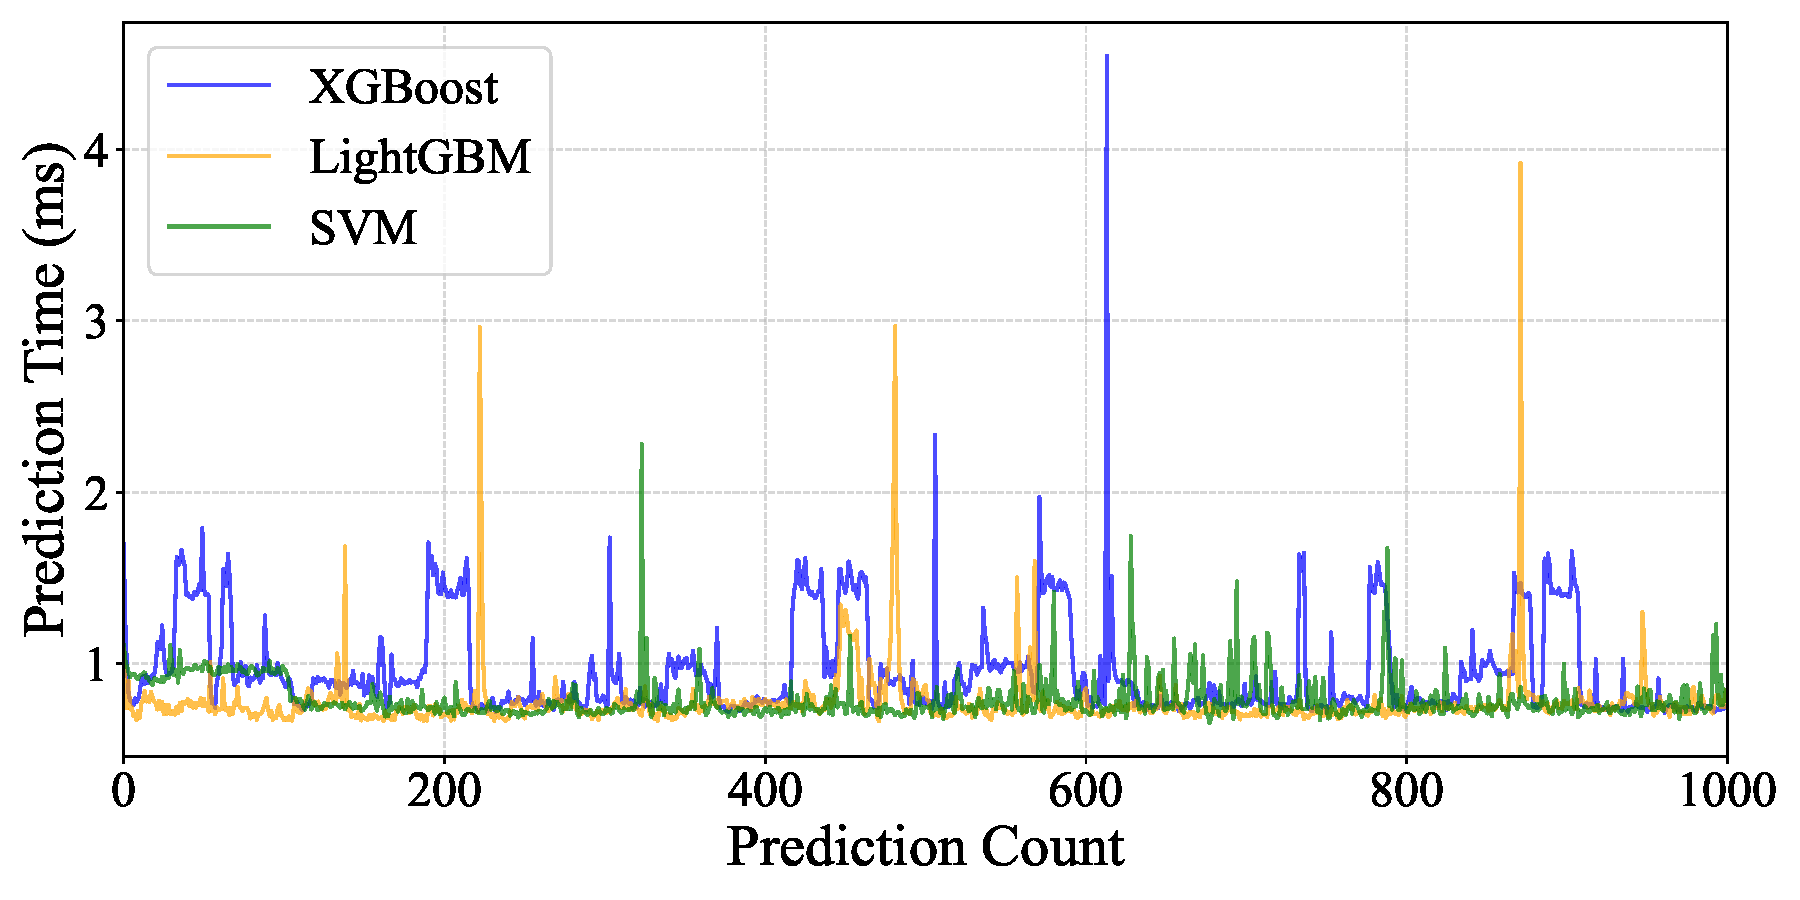
\includegraphics[width=0.48\textwidth]{./figures/PredictionTimeCostsLine.pdf}
    \caption{Line chart comparing the prediction time costs.}
    \label{PredictionTimeCostsLine}
\end{figure}

\begin{figure}[!t]
    \centering
    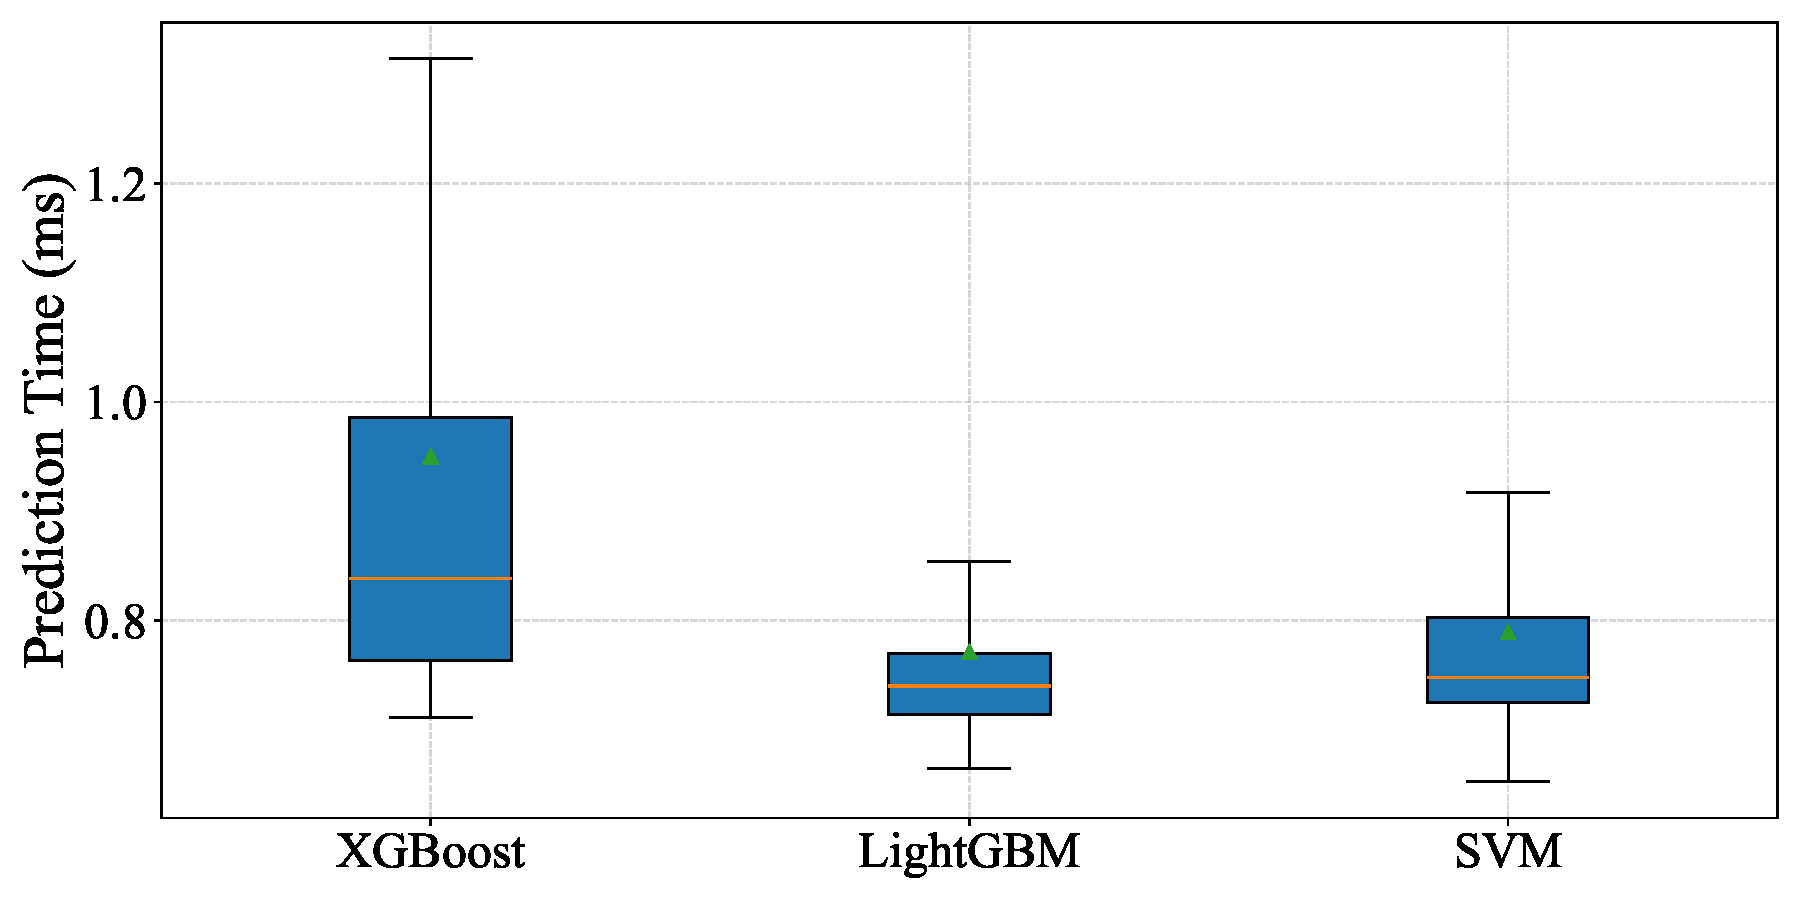
\includegraphics[width=0.48\textwidth]{./figures/PredictionTimeCostsBox.pdf}
    \caption{Boxplot comparing the prediction time costs.}
    \label{PredictionTimeCostsBox}
\end{figure}

\subsection{Evaluation Metrics}

\noindent To comprehensively assess the performance of various monitoring schemes---including fixed-threshold and machine learning-based adaptive thresholding methods---under identical traffic conditions, three core evaluation metrics are defined. 
These metrics respectively measure the reporting error rate, communication overhead, and overall system cost, enabling quantitative comparison across key dimensions.

The reporting error rate $\varepsilon$ evaluates the accuracy of reported traffic statistics and is formally defined as:
\begin{equation}
    \varepsilon = \frac{1}{N} \sum_{i=1}^{N} \left| \frac{r_{i}^{reported} - r_{i}^{true}}{r_{i}^{true}} \right|,
\end{equation}
where $N$ denotes the number of reporting events, and $r_{i}^{reported}$ and $r_{i}^{true}$ represent the reported and actual rates, respectively, at the $i$-th instance. 
This metric corresponds to the average of relative errors across all reporting events. 
A lower value of $\varepsilon$ indicates a higher fidelity of the monitoring system in capturing the true network dynamics and is thus a critical measure of monitoring accuracy.

The communication overhead $C$ quantifies the control plane burden introduced by monitoring, defined as the average number of reports per unit time. 
The total number of reporting events during the test period is divided by the total test duration to yield the raw reporting frequency. 
For consistency with the error metric and for multi-objective optimization, the overhead is normalized with respect to a predefined upper bound $C_{max}=50$ (i.e., a maximum of 50 reports per second):
\begin{equation}
    C_{norm} = \frac{C_{raw}}{C_{max}},
\end{equation}
where the raw overhead $C_{raw}$ is computed as:
\begin{equation}
    C_{raw} = \frac{R}{T},
\end{equation}
with $R$ denoting the total number of reporting events during the evaluation period, and $T$ representing the total duration. 
A lower $C_{norm}$ implies a reduced communication burden, which alleviates the processing pressure on the controller and reduces bandwidth consumption.

To balance monitoring accuracy against communication efficiency, a composite metric $\text{Cost}$ is introduced, defined as a weighted sum of the reporting error $\varepsilon$ and the normalized communication overhead $C_{norm}$:
\begin{equation}
    \text{Cost} = \alpha \cdot \varepsilon + \beta \cdot C_{norm},
\end{equation}
where $\alpha$ and $\beta$ are weighting coefficients corresponding to the relative importance of accuracy and overhead.
For consistency with dataset construction, the values $\alpha = 0.6$ and $\beta = 0.4$ are adopted, reflecting a greater emphasis on monitoring precision. 
Minimizing $\text{Cost}$ ensures that the system achieves a favorable trade-off between accuracy and efficiency, aligning with practical deployment objectives.

During the evaluation process, each monitoring scheme is independently tested over a 30-second period under identical traffic inputs. 
This uniform test condition eliminates external variability and ensures fair comparability across different methods. 
The proposed tri-metric framework allows for multi-faceted, systematic assessment of each scheme in terms of accuracy, efficiency, and overall cost-effectiveness, thereby providing a robust analytical foundation for subsequent performance analysis.

\subsection{Experimental Results and Analysis}

\noindent This section presents and analyzes the experimental results of MAT4PM across several key dimensions, including its impact on throughput performance and the effectiveness of the dynamic threshold control strategy powered by machine learning models. 
\rev{In addition to reporting mean values, statistical variability is explicitly characterized through confidence intervals (CIs) and error bars to provide a more comprehensive assessment of performance stability.}

Figure~\ref{loss_mbps} illustrates the variation in switch throughput after the integration of the MAT4PM monitoring mechanism. 
To evaluate the potential performance overhead introduced by the monitoring logic on the data plane, TCP throughput was measured using the iPerf tool in repeated trials. 
Each trial was conducted under two conditions: without the monitoring module (baseline) and with MAT4PM enabled while monitoring varying proportions of traffic. 
In the testbed, Host~2 operated as an iPerf server receiving a continuous 30-second TCP stream from Host~1, while the MAT4PM logic was deployed on the intermediate switch, Switch~2. 
By adjusting the percentage of monitored flows, the impact on overall throughput was observed. 
The blue dashed line in the figure represents the maximum throughput achieved without monitoring, while the orange solid line shows the measured throughput under different monitoring intensities. 
As the monitored traffic ratio increases, a gradual decline in throughput is observed. 
When 100\% of the traffic is monitored, throughput of MAT4PM decreases to 21.0 Mbps, approximately 13.2\% lower than the baseline of 24.2 Mbps. 
% This performance degradation is primarily attributed to the additional computational cost introduced by monitoring logic in the ingress pipeline, where each monitored packet triggers read and write operations across four registers (responsible for storing thresholds, byte counters, packet counters, and reporting timestamps). 
\rev{This performance degradation is primarily attributed to the additional computational cost introduced by the monitoring logic in the ingress pipeline. 
Each monitored packet triggers read and write operations across four registers, which store thresholds, byte counters, packet counters, and reporting timestamps.} 
As the monitoring coverage expands, the frequency of register access increases, which in turn negatively impacts the packet processing rate of the switch. 
Notably, this throughput impact aligns with state-of-the-art monitoring frameworks such as PPM \cite{10623873} and FlowStalker \cite{8761197}, which exhibit 13.05\% and 12\% throughput reduction under full traffic coverage.

\begin{figure}[!t]
    \centering
    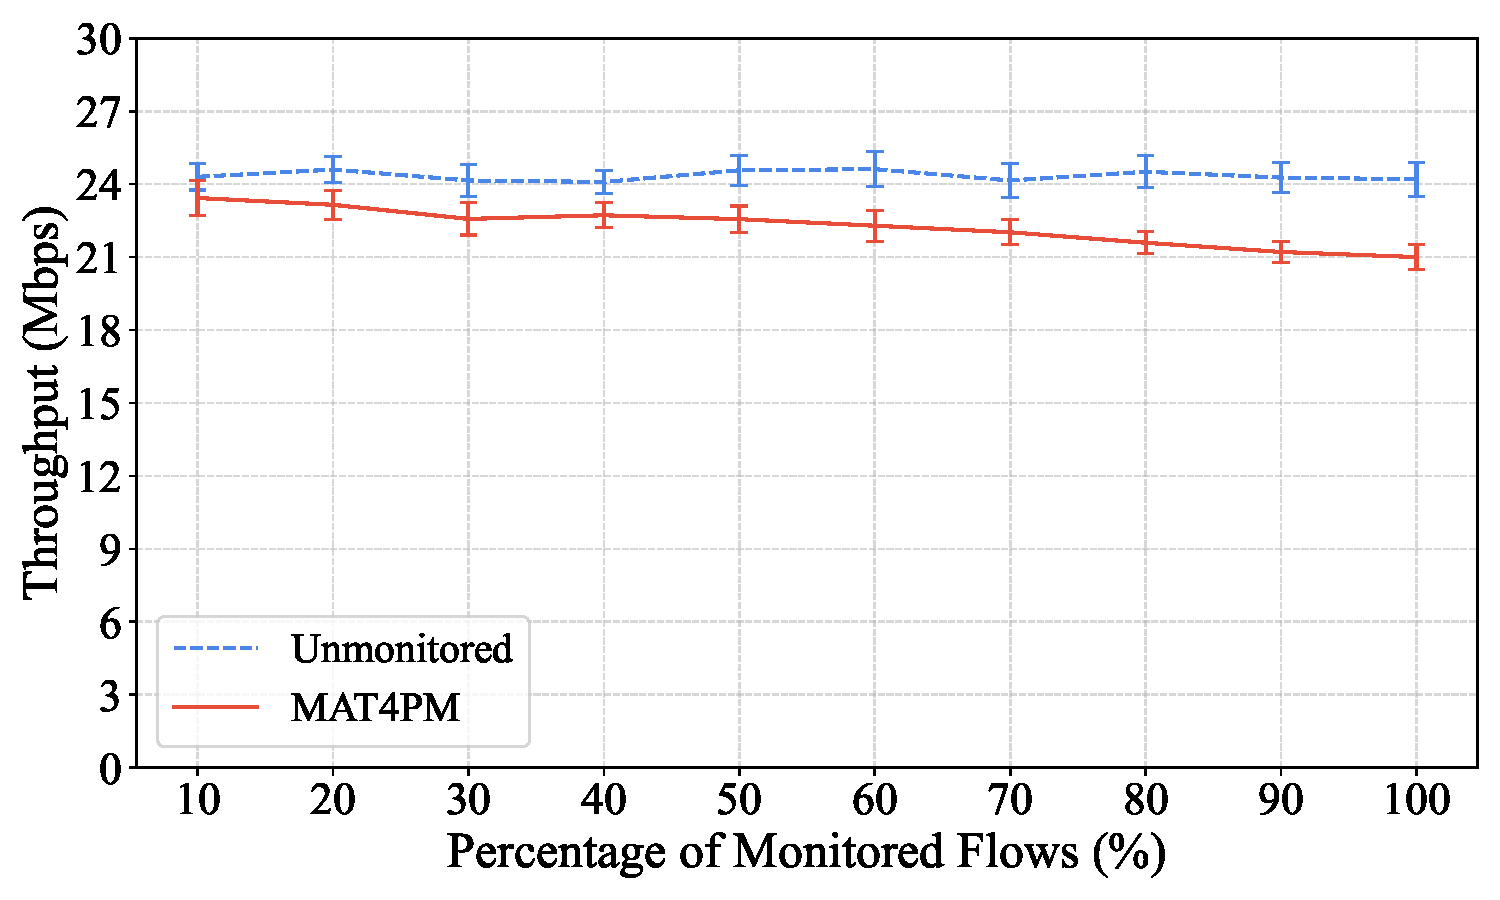
\includegraphics[width=0.49\textwidth]{./figures/loss_mbps.pdf}
    \caption{The impact of MAT4PM on throughput.}
    \label{loss_mbps}
\end{figure}

The subsequent experiments aim to evaluate the performance of machine learning-based dynamic threshold control strategies in real traffic scenarios, focusing on metrics including monitoring error, communication overhead, and overall cost. 
In this evaluation, Scapy was employed to generate a single flow with dynamic characteristics over a 30-second period, where the transmission rate changed every 5 seconds. 
Three dynamic threshold strategies based on machine learning models (XGBoost, LightGBM, and SVM) were compared against three fixed threshold baselines (with reporting intervals of 500~ms, 1000~ms, and 2000~ms).

Figure~\ref{monitoring} exemplifies the monitoring process under the XGBoost-based dynamic strategy. 
In this test, the traffic rates were set to 4 Mbps (0--5~s), 5.5 Mbps (5--10~s), 7.5 Mbps (10--15~s), 6 Mbps (15--20~s), 4 Mbps (20--25~s), and 7 Mbps (25--30~s). 
The blue solid line denotes the actual traffic rate, while the red dashed line indicates the corresponding reported rate. 
Overall, the two curves show close alignment across the entire test duration, indicating a high level of tracking accuracy. 
The system adaptively adjusts its reporting frequency based on traffic intensity. 
For instance, during the low-load period of 0--5 seconds, monitoring data were reported 12 times, whereas in the high-load interval of 10--15 seconds, the reporting frequency increased to 19. 
This behavior demonstrates a strong capacity for dynamic adaptation.

\begin{figure}[!t]
    \centering
    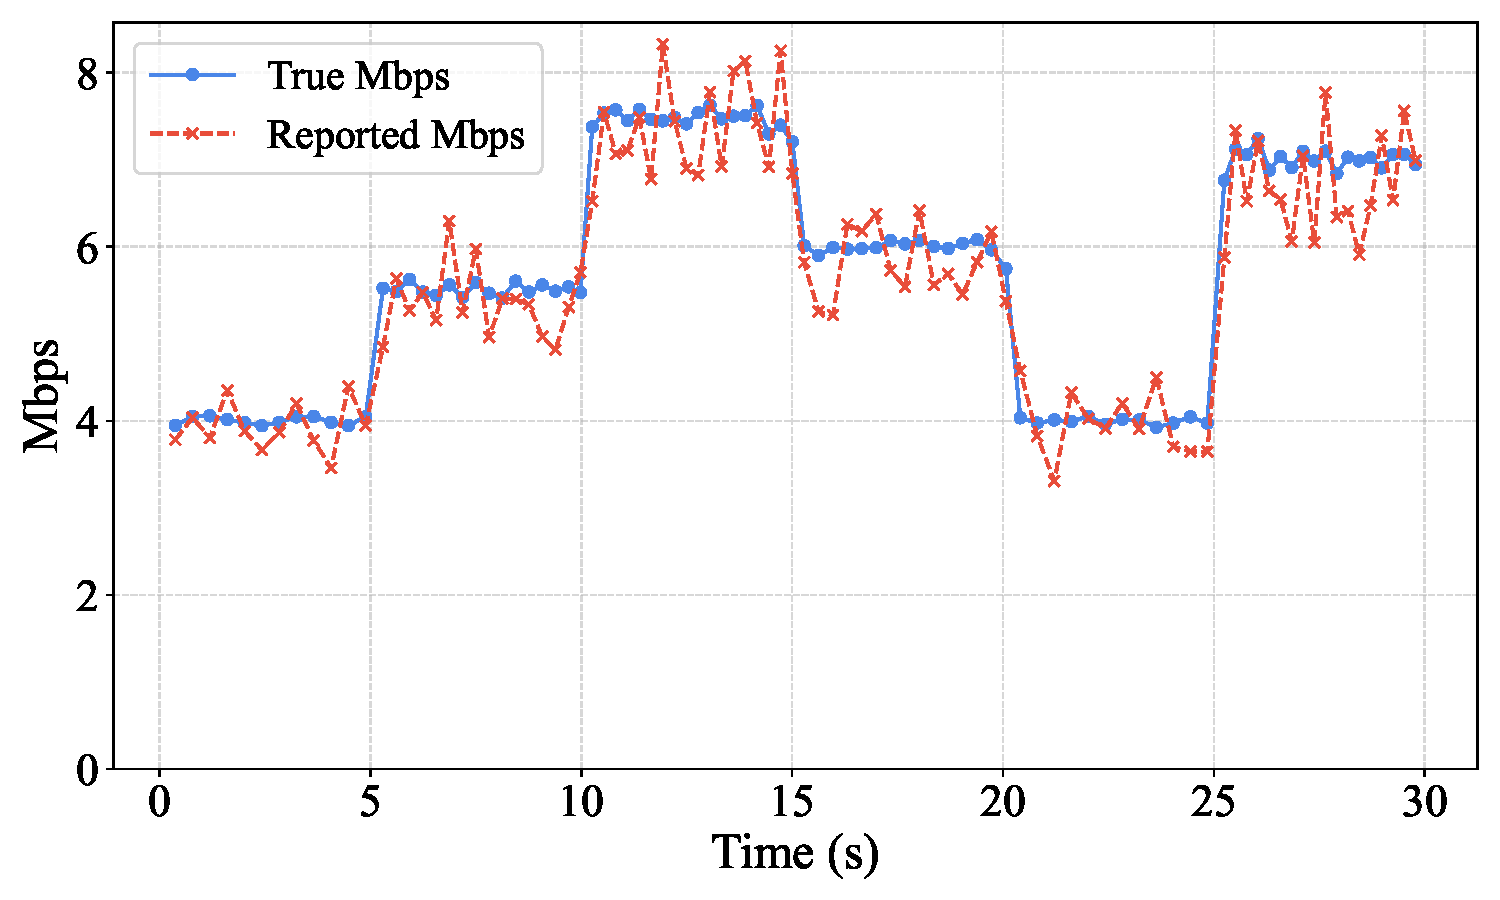
\includegraphics[width=0.49\textwidth]{./figures/monitoring.pdf}
    \caption{The monitoring process based on the XGBoost model.}
    \label{monitoring}
\end{figure}

To provide a consolidated view of monitoring performance, Table~\ref{summary_table} summarizes the key evaluation metrics---average monitoring error, reporting frequency, and total cost---for all six schemes. 
\rev{To characterize statistical variability, the reported monitoring error and total cost are expressed as mean values accompanied by their corresponding 95\% confidence intervals, computed over repeated measurements. 
This presentation provides insights into both average performance and result stability.}

\begin{table*}[!t]
    \centering
    \caption{Comparison of monitoring schemes in terms of error, reporting frequency, and total cost \rev{(mean $\pm$ 95\% CI)}.}
    \label{summary_table}
    \begin{tabular}{p{0.22\textwidth}<{\centering} p{0.18\textwidth}<{\centering} p{0.18\textwidth}<{\centering} p{0.16\textwidth}<{\centering}}
        \toprule
        \textbf{Scheme} & \textbf{Average Error (\%)} & \textbf{Reports per Second} & \textbf{Total Cost} \\
        \midrule
        \textbf{Fixed-500ms}
            & $ 9.1 \pm 0.31$
            & 1.967
            & $0.0703 \pm 0.0019$ \\
        \textbf{Fixed-1000ms}
            & $10.8 \pm 0.35$
            & 0.967
            & $0.0725 \pm 0.0021 $ \\
        \textbf{Fixed-2000ms}
            & $11.6 \pm 0.42$
            & \textbf{0.467}
            & $0.0733 \pm 0.0025$ \\
        \textbf{XGBoost}
            & $\mathbf{7.0 \pm 0.26}$
            & 3.033
            & $0.0663 \pm 0.0015$ \\
        \textbf{LightGBM}
            & $7.3 \pm 0.24$
            & 2.800
            & $\mathbf{0.0662 \pm 0.0015}$ \\
        \textbf{SVM}
            & $7.5 \pm 0.29$
            & 2.767
            & $0.0671 \pm 0.0018$ \\
        \bottomrule
    \end{tabular}
\end{table*}

These metrics are further examined and visualized in the subsequent figures. Figure~\ref{errors} presents the average monitoring error across the six schemes over the 30-second test duration. 
The fixed threshold configurations (500 ms, 1000 ms, and 2000 ms) yielded average errors of 9.1\%, 10.8\%, and 11.6\%, respectively. 
In contrast, the \mbox{XGBoost-}, \mbox{LightGBM-}, and SVM-based dynamic strategies achieved lower errors of 7.0\%, 7.3\%, and 7.5\%, respectively. 
\rev{In addition to mean error values, 95\% confidence intervals are depicted using error bars to reflect the variability of monitoring performance across repeated trials.} 
These results confirm the superiority of dynamic threshold control in improving monitoring accuracy compared to static schemes, \rev{and dynamic schemes exhibit relatively narrow confidence intervals, which indicates the stability and reliability of dynamic threshold control.}

\begin{figure}[!t]
    \centering
    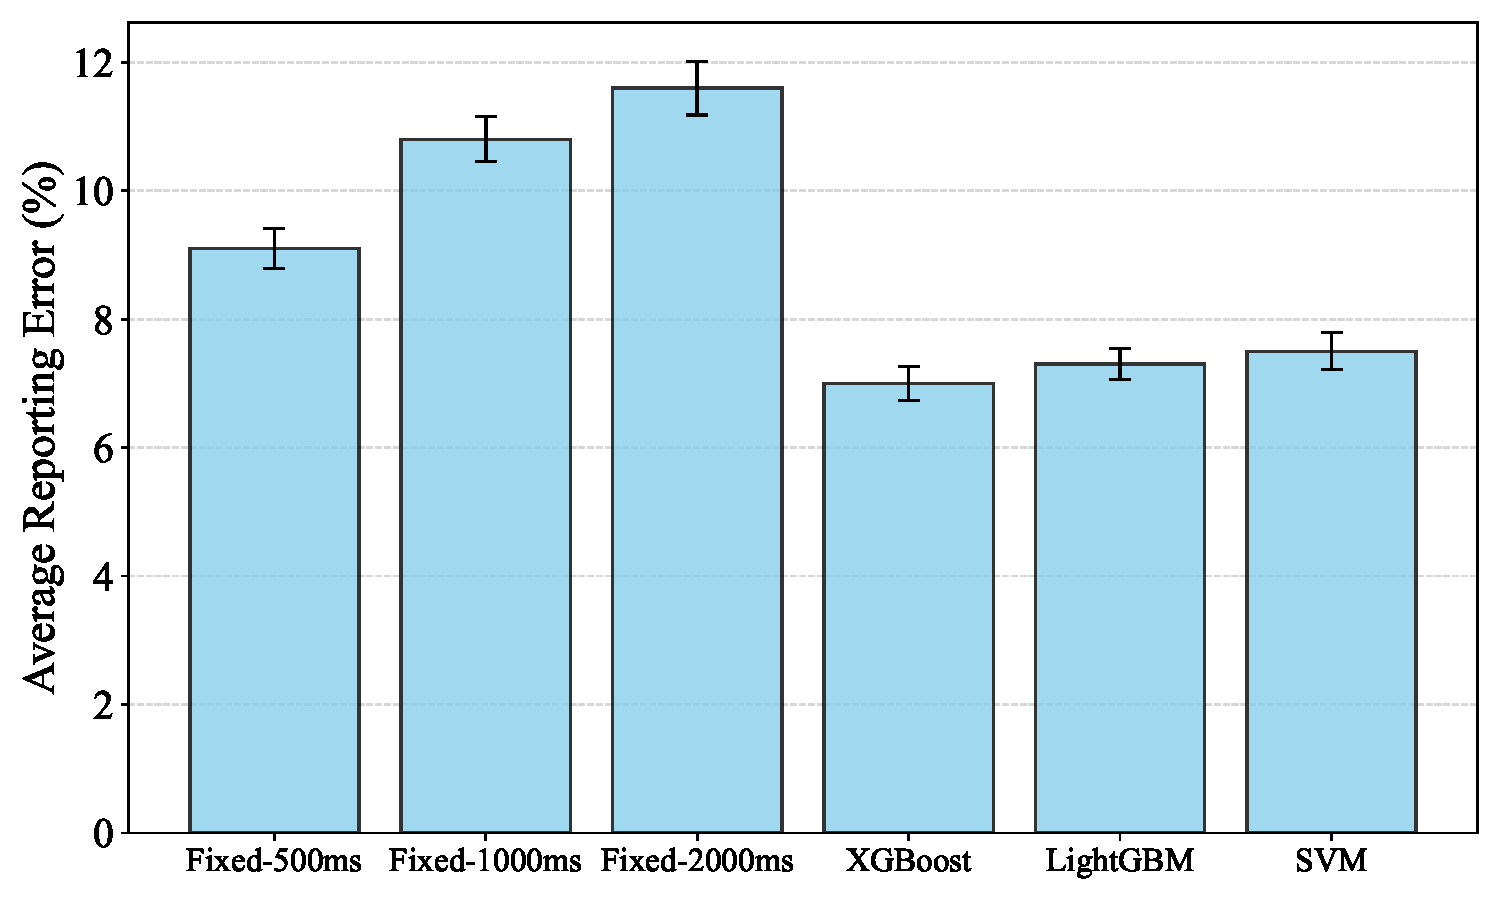
\includegraphics[width=0.49\textwidth]{./figures/errors.pdf}
    \caption{Average monitoring error of different schemes. \rev{Error bars indicate the 95\% CI.}}
    \label{errors}
\end{figure}

Figure~\ref{rps} provides the average number of reports per second for each scheme during the test period. 
The fixed interval strategies resulted in reporting rates of 1.967, 0.967, and 0.467 reports per second for the 500~ms, 1000~ms, and 2000~ms thresholds, respectively. 
It is important to note that a 500~ms reporting threshold does not guarantee an exact report every 500~ms. 
Instead, each report must be triggered by the arrival of at least one data packet; thus, the actual interval between consecutive reports is typically greater than or equal to the configured threshold. 
For instance, with a 500~ms threshold over a 30-second test duration, the total number of triggered reports was 59 rather than 60, yielding an observed average of 1.967 reports per second. 
The machine learning-based dynamic schemes achieved higher average reporting rates, with XGBoost, LightGBM, and SVM reporting monitoring data at 3.033, 2.800, and 2.767 times per second, respectively. 
Although these strategies incur increased communication frequency, they enable finer-grained monitoring under high traffic loads, thereby contributing to improved accuracy.

\begin{figure}[!t]
    \centering
    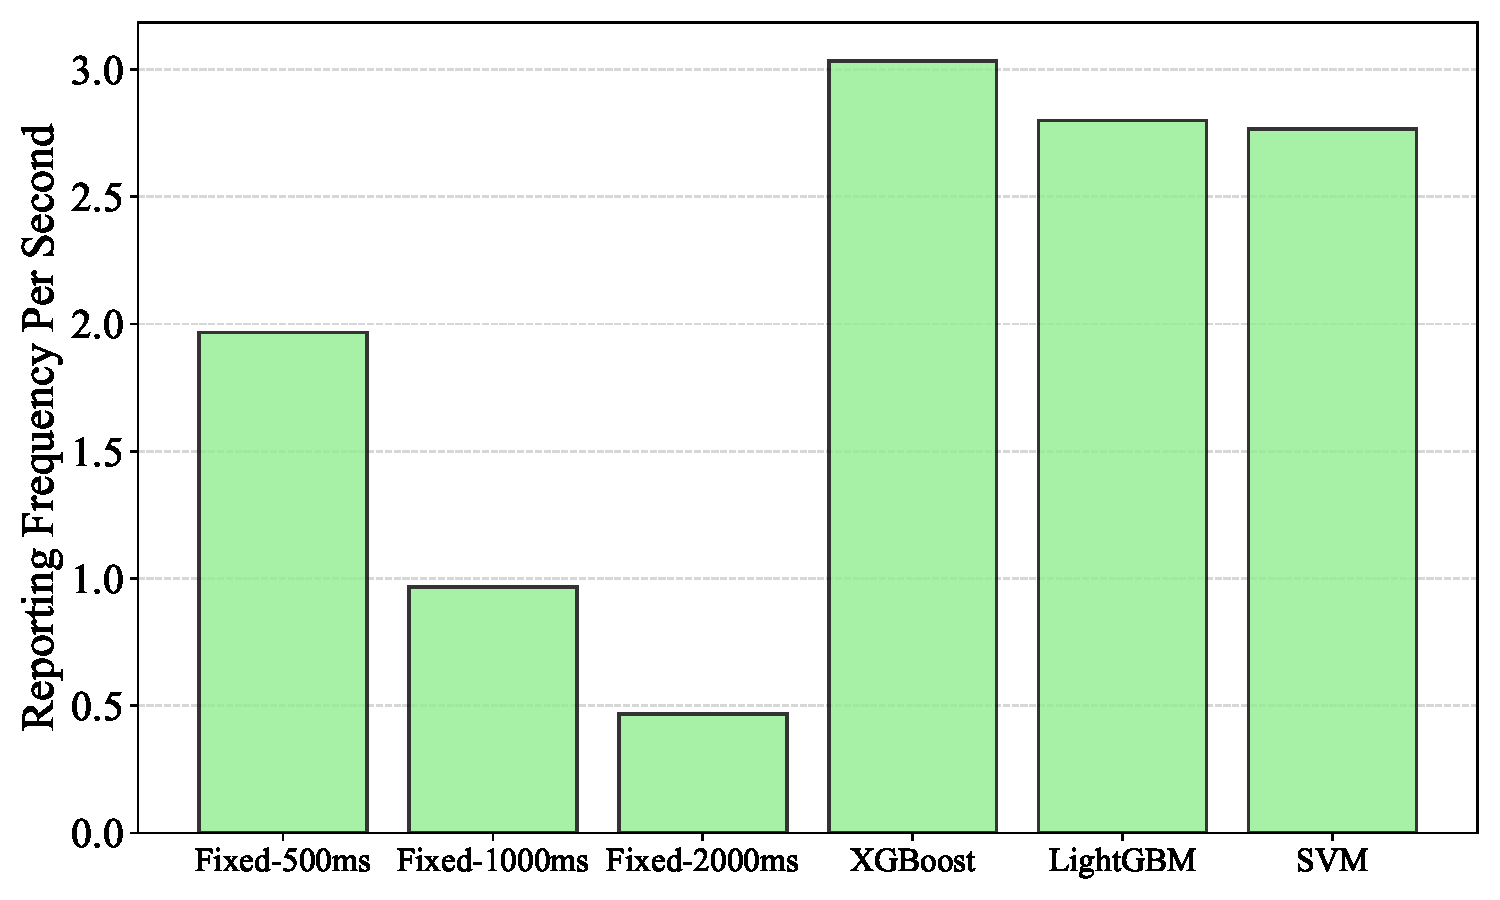
\includegraphics[width=0.49\textwidth]{./figures/rps.pdf}
    \caption{Average reporting frequency per second of different schemes.}
    \label{rps}
\end{figure}

To assess the trade-off between monitoring accuracy and communication cost, Figure~\ref{costs} reports the total cost for each scheme using weighted coefficients $\alpha=0.6$ and $\beta=0.4$. 
The fixed threshold strategies yielded total costs of 0.0703, 0.0725, and 0.0733 for the 500 ms, 1000 ms, and 2000 ms configurations, respectively. In comparison, the \mbox{XGBoost-,} \mbox{LightGBM-,} and SVM-based dynamic approaches achieved lower total costs of 0.0663, 0.0662, and 0.0671, respectively. 
These results reinforce the advantage of incorporating machine learning in striking a more favorable balance between accuracy and communication overhead, thereby reducing overall monitoring cost.

\begin{figure}[!t]
    \centering
    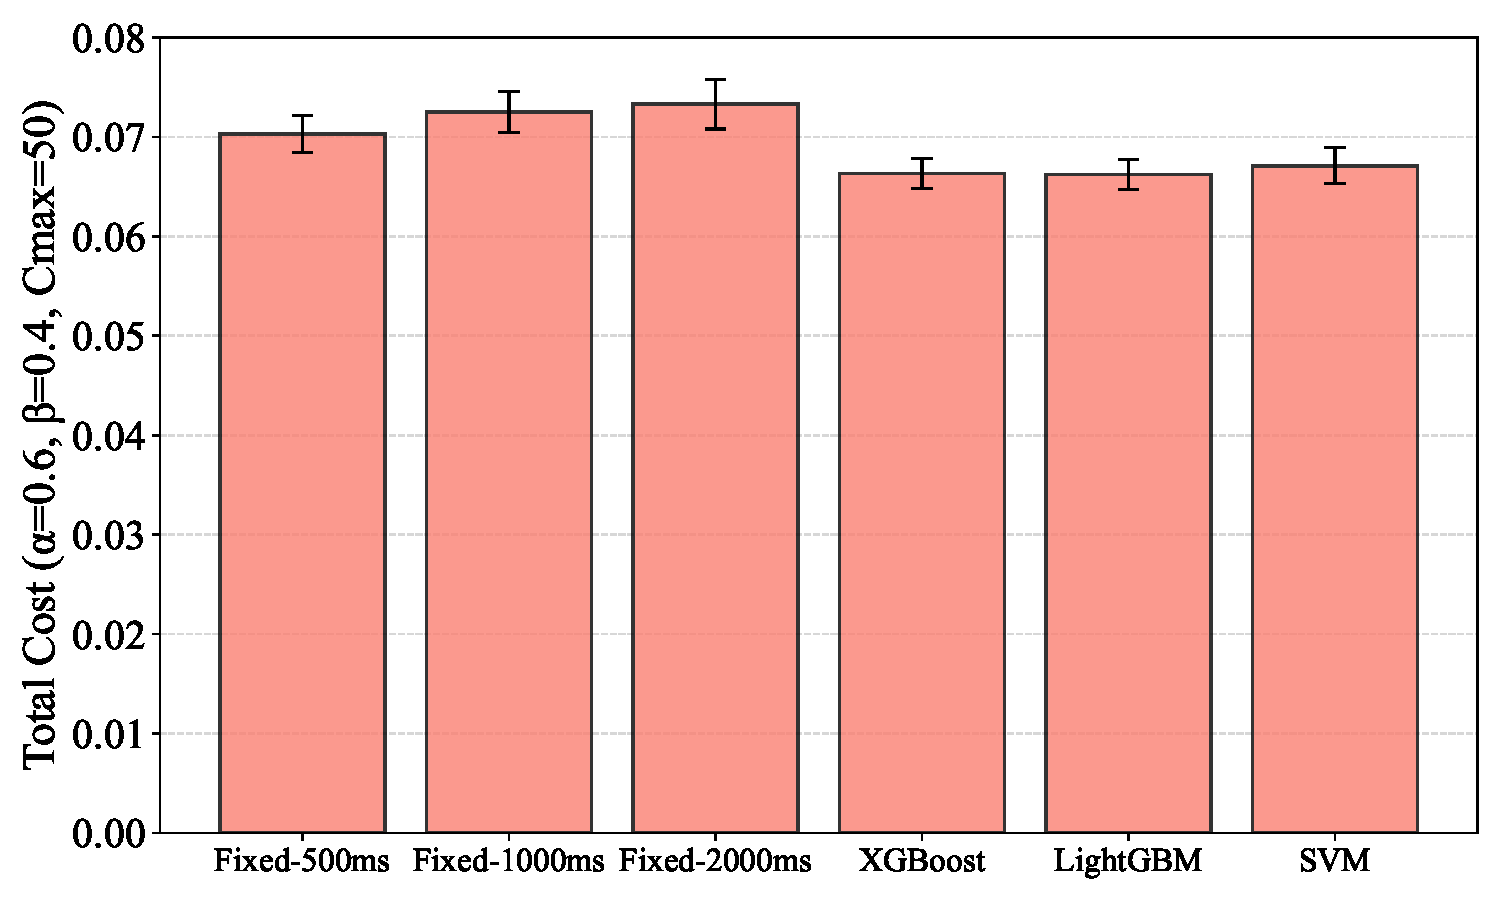
\includegraphics[width=0.49\textwidth]{./figures/costs.pdf}
    \caption{Total cost comparison among different monitoring schemes. \rev{Error bars indicate the 95\% CI.}}
    \label{costs}
\end{figure}

\rev{
Although Table~\ref{summary_table} reports quantitative differences among the three machine learning-based strategies, the primary objective of this evaluation is not to identify a universally optimal learning algorithm, but rather to demonstrate the effectiveness and robustness of machine learning-driven adaptive threshold control as a general paradigm.
}

\rev{
The three models considered in this study, namely XGBoost, LightGBM, and SVM, are selected as representative and widely adopted regression techniques with distinct learning characteristics. 
Tree-based ensemble models such as XGBoost and LightGBM are known for their strong capability in capturing nonlinear feature interactions and piecewise decision boundaries, which is particularly suitable for modeling the nonlinear relationship between traffic intensity and optimal monitoring thresholds~\cite{XGBoost,LightGBM}. 
This property partially explains why the XGBoost-based strategy achieves the lowest average monitoring error, while LightGBM attains the minimum total cost by maintaining a slightly lower reporting frequency under similar accuracy levels.
}

\rev{
In contrast, the SVM-based strategy exhibits marginally higher error and cost compared to the tree-based models. 
This behavior can be attributed to the sensitivity of kernel-based methods to hyperparameter selection and their limited flexibility in approximating abrupt changes when traffic patterns vary rapidly over short time scales~\cite{SVMs}. 
Nevertheless, the performance gap among the three models remains relatively small, and all machine learning-based approaches consistently outperform the fixed-threshold baselines on both average error and total cost.
}

\rev{
These observations suggest that the overall performance gains primarily stem from the introduction of adaptive, data-driven threshold adjustment, rather than reliance on a specific learning algorithm. 
Consequently, the proposed framework is compatible with a wide range of regression models, allowing practitioners to select learning techniques based on deployment constraints, interpretability requirements, or computational considerations.
}

\subsection{\rev{Scalability Analysis}}

\noindent \rev{
The proposed framework introduces machine learning driven adaptive threshold computation at the control plane, which inevitably incurs additional computational overhead compared to purely rule based monitoring schemes. 
To evaluate the scalability of the system under increasing monitoring scale, controller CPU utilization is examined along two dimensions: the number of concurrent flows and the number of monitored switches.
}

\subsubsection{\rev{Impact of Number of Flows}}

\rev{
The first experiment investigates the effect of flow scale on controller CPU usage. 
The experiment is conducted on the linear two switch topology illustrated in Figure~\ref{topo}, where telemetry data are collected from a single monitored switch. 
The number of active flows is gradually increased from 10 to 500, while all other parameters remain unchanged.
}

\rev{
Table~\ref{tab:cpu_flow} summarizes the statistical characteristics of controller CPU utilization under different flow counts, including the average, median, peak, minimum, and standard deviation. 
As shown in the table, CPU utilization increases steadily with the number of flows, rising from an average of 7.53\% at 10 flows to 64.0\% at 100 flows. 
Beyond 200 flows, the average CPU usage approaches a plateau around 72\%, and no further linear growth is observed even when the number of flows increases to 500.
}

\begin{table*}[!t]
    \centering
    \caption{\rev{Controller CPU utilization under different numbers of monitored flows.}}
    \label{tab:cpu_flow}
    \begin{tabular}{p{0.16\textwidth}<{\centering}
                    p{0.09\textwidth}<{\centering}
                    p{0.09\textwidth}<{\centering}
                    p{0.09\textwidth}<{\centering}
                    p{0.09\textwidth}<{\centering}
                    p{0.09\textwidth}<{\centering}}
        \toprule
        \textbf{\rev{Number of Flows}} & \textbf{\rev{Mean (\%)}} & \textbf{\rev{Median (\%)}} & \textbf{\rev{Peak (\%)}} & \textbf{\rev{Min (\%)}} & \textbf{\rev{Std. Dev.}} \\
        \midrule
        \rev{10 } & \rev{7.53 } & \rev{7.58 } & \rev{10.74} & \rev{3.79 } & \rev{1.74} \\
        \rev{20 } & \rev{14.28} & \rev{13.90} & \rev{18.32} & \rev{9.48 } & \rev{2.2 } \\
        \rev{50 } & \rev{34.05} & \rev{34.58} & \rev{42.33} & \rev{26.90} & \rev{3.57} \\
        \rev{100} & \rev{64.0 } & \rev{64.44} & \rev{76.45} & \rev{44.23} & \rev{7.38} \\
        \rev{200} & \rev{71.65} & \rev{71.71} & \rev{79.61} & \rev{61.28} & \rev{5.25} \\
        \rev{500} & \rev{73.07} & \rev{73.82} & \rev{80.24} & \rev{58.76} & \rev{4.53} \\
        \bottomrule
    \end{tabular}
\end{table*}

\rev{
To further illustrate the distribution and variability of CPU usage, Figure~\ref{cpu_usage_flow} presents boxplots of controller CPU utilization under different flow counts. 
The results indicate that both the median and interquartile range increase rapidly up to 100 flows, followed by a clear saturation trend. 
This behavior suggests that the controller reaches a stable operating regime in which available CPU resources become the dominant limiting factor.
}

\begin{figure}[!t]
    \centering
    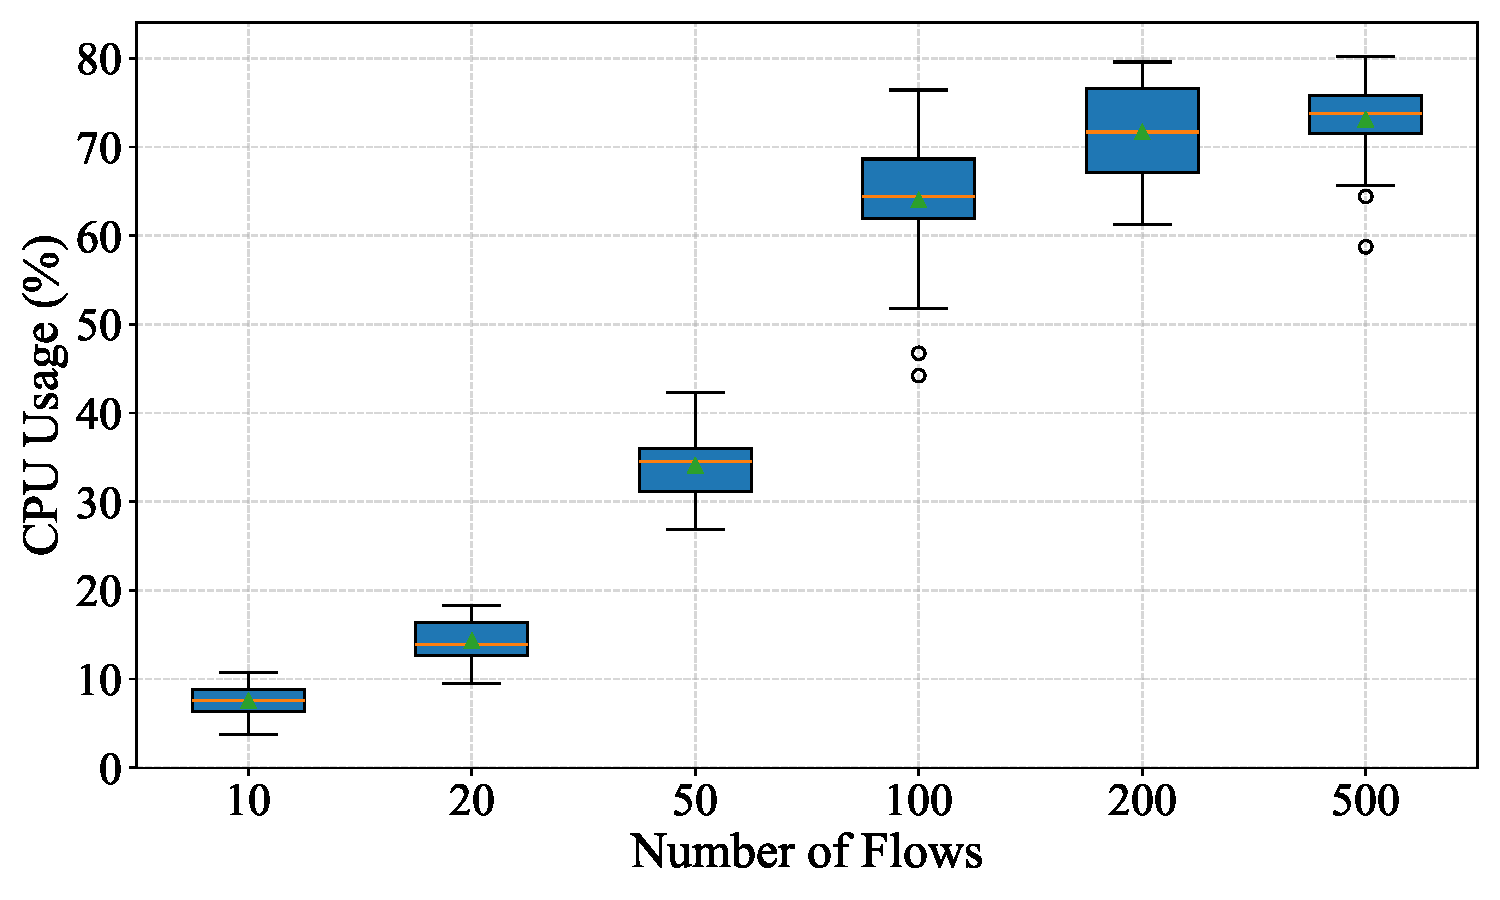
\includegraphics[width=0.49\textwidth]{./figures/cpu_usage_flow.pdf}
    \caption{\rev{Distribution of controller CPU usage under varying numbers of monitored flows.}}
    \label{cpu_usage_flow}
\end{figure}

\subsubsection{\rev{Impact of Number of Switches}}

\rev{
The second experiment evaluates scalability with respect to network size by increasing the number of monitored switches. 
The experiment linearly scales the topology from one to five monitored switches. 
Figure~\ref{topo} illustrates the baseline two-switch case. 
The number of active flows is fixed at 40, and the controller concurrently processes telemetry feedback from all monitored switches.
%Starting from the baseline topology shown in Figure~\ref{topo}, additional switches are incrementally added to form linear topologies with one to five monitored switches. 
%Throughout this experiment, the number of active flows is fixed at 40, and the controller concurrently processes telemetry feedback from all monitored switches.
}

\rev{
Table~\ref{tab:cpu_switch} reports the controller CPU utilization statistics under different numbers of switches. 
The results show that average CPU usage increases sharply when the number of switches grows from one to three, rising from 14.75\% to 65.76\%. 
When four or five switches are monitored concurrently, CPU utilization stabilizes at approximately 71\%, exhibiting a similar saturation effect to that observed in the flow scaling experiment.
}

\begin{table*}[!t]
    \centering
    \caption{\rev{Controller CPU utilization under different numbers of monitored switches.}}
    \label{tab:cpu_switch}
    \begin{tabular}{p{0.16\textwidth}<{\centering}
                    p{0.09\textwidth}<{\centering}
                    p{0.09\textwidth}<{\centering}
                    p{0.09\textwidth}<{\centering}
                    p{0.09\textwidth}<{\centering}
                    p{0.09\textwidth}<{\centering}}
        \toprule
        \textbf{\rev{Number of Switches}} & \textbf{\rev{Mean (\%)}} & \textbf{\rev{Median (\%)}} & \textbf{\rev{Peak (\%)}} & \textbf{\rev{Min (\%)}} & \textbf{\rev{Std. Dev.}} \\
        \midrule
        \rev{1} & \rev{14.75} & \rev{14.22} & \rev{22.11} & \rev{8.85 } & \rev{3.77} \\
        \rev{2} & \rev{40.84} & \rev{42.96} & \rev{48.02} & \rev{20.64} & \rev{5.86} \\
        \rev{3} & \rev{65.76} & \rev{67.89} & \rev{76.45} & \rev{44.86} & \rev{7.98} \\
        \rev{4} & \rev{71.57} & \rev{71.66} & \rev{79.61} & \rev{65.08} & \rev{3.99} \\
        \rev{5} & \rev{71.45} & \rev{71.39} & \rev{80.24} & \rev{65.06} & \rev{3.68} \\
        \bottomrule
    \end{tabular}
\end{table*}

\rev{
Figure~\ref{cpu_usage_sw} depicts the corresponding boxplots of CPU usage. 
The results confirm that controller load grows rapidly with the number of monitored switches but converges to a stable upper bound once system resources become fully utilized.
}

\begin{figure}[!t]
    \centering
    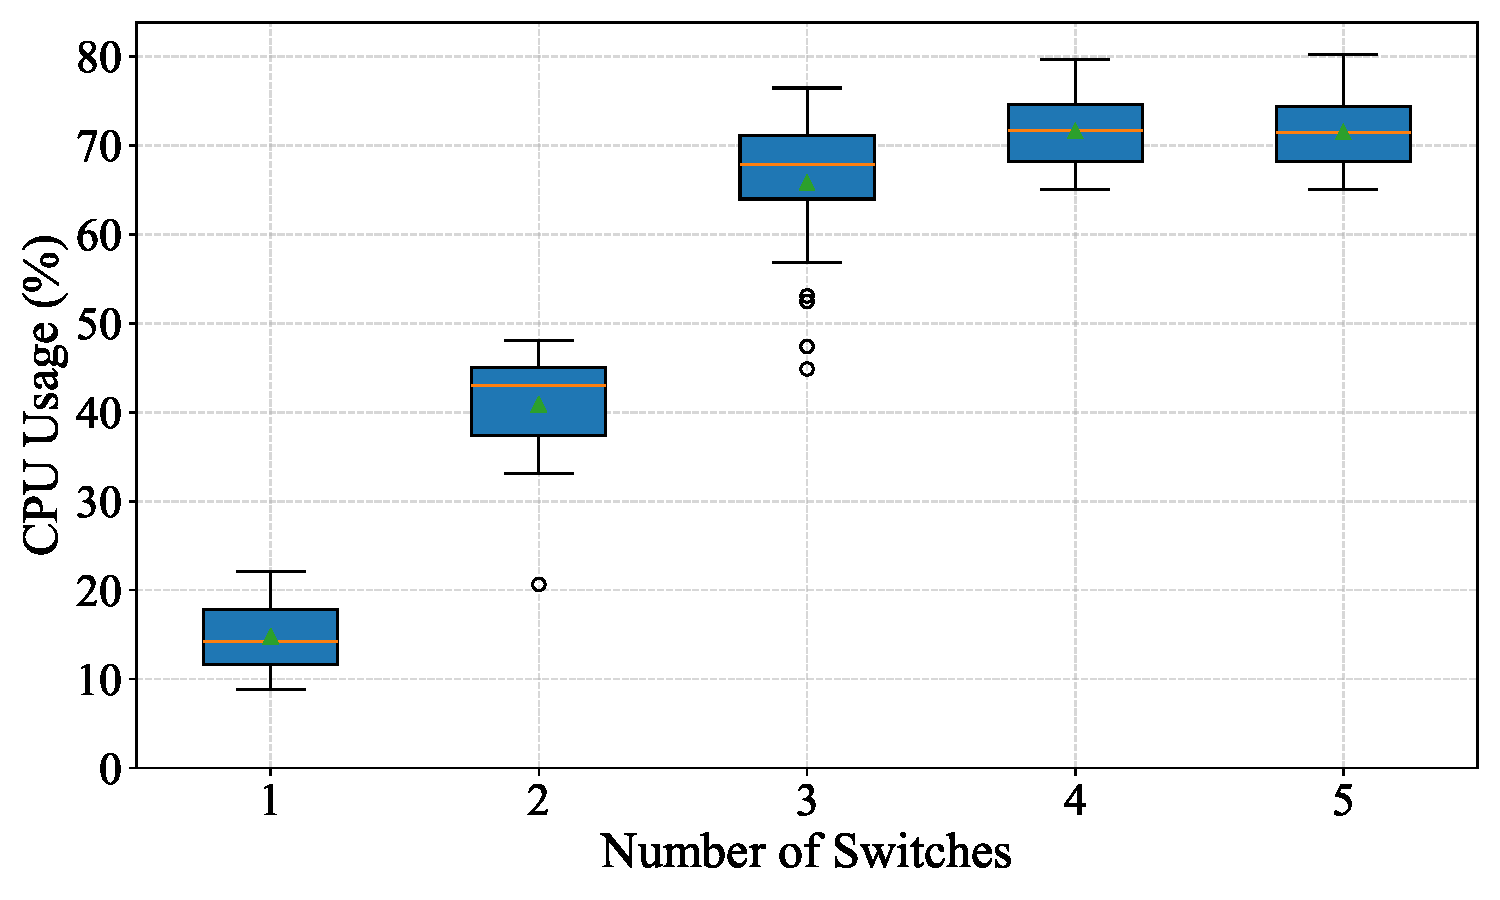
\includegraphics[width=0.49\textwidth]{./figures/cpu_usage_sw.pdf}
    \caption{\rev{Distribution of controller CPU usage under varying numbers of monitored switches.}}
    \label{cpu_usage_sw}
\end{figure}

\subsubsection{\rev{Discussion}}

\rev{
Across both experiments, controller CPU utilization converges to a similar upper bound of approximately 70\%. 
This phenomenon is primarily attributed to the limited computational resources of the experimental environment, where CPU capacity is concurrently consumed by network emulation, traffic generation, machine learning inference, and operating system processes. 
Once the CPU becomes saturated, additional increases in flows or switches do not translate into proportional increases in observed utilization.
}

\rev{
Importantly, this behavior reflects a limitation of the software based testbed rather than an inherent scalability bottleneck of the proposed framework. 
In practical deployments with hardware controllers or dedicated control plane resources, the same adaptive monitoring logic is expected to scale to substantially larger numbers of flows and switches. 
Therefore, the observed saturation indicates stable system behavior under resource constrained conditions, while suggesting that scalability can be further improved with more powerful control plane infrastructure.
}

\rev{
Metrics such as P4Runtime RPC rate, register write latency, and end to end monitoring latency are not separately reported in this evaluation. 
These metrics are tightly coupled with controller CPU load in the adopted software based testbed, and their behavior is largely dominated by overall system resource contention rather than protocol level bottlenecks. 
As a result, controller CPU utilization serves as a representative and conservative indicator of scalability under increasing monitoring scale in the considered environment.
}

\section{Conclusions and Future Works}
\label{sec5}

\noindent This paper presents MAT4PM, an active monitoring framework that integrates machine learning based control plane with a programmable data plane to enable adaptive and fine-grained threshold control in SDN. 
% The proposed system leverages the P4 language to implement lightweight monitoring logic on the switch side, in conjunction with a controller-side learning module that dynamically adjusts monitoring intervals, coordinated via a P4Runtime-based feedback interface. 
\rev{The system leverages the P4 language to implement lightweight monitoring logic on the switch side. 
A controller-side learning module dynamically adjusts monitoring intervals through a P4Runtime-based feedback interface.} 
This control interface connects the data and control planes, enabling timely synchronization between observed traffic conditions and policy updates. 
By introducing a composite cost function that jointly considers monitoring accuracy and communication overhead, MAT4PM effectively balances performance and efficiency through event-driven threshold updates.

Comprehensive evaluations in the Mininet environment and on BMv2 software switches demonstrate that the dynamic threshold schemes powered by machine learning models consistently outperform traditional fixed-threshold baselines across multiple metrics. 
Specifically, the dynamic schemes reduce average monitoring error from 9.1\% to 7.0\%, improve reporting precision, and lower overall monitoring cost by 5.6\%. 
The inference delay of the models remains below the millisecond scale, and resource consumption is minimal, indicating the practical deployability and scalability of the proposed approach in real-world network conditions.

\rev{
Future research directions include several complementary extensions to further enhance the practicality and robustness of MAT4PM. 
First, reinforcement learning and other online or self-supervised learning paradigms will be investigated to reduce or eliminate the reliance on offline labeled datasets, enabling continuous adaptation under evolving traffic conditions without manual data annotation. 
Second, deployment on physical programmable hardware platforms will be explored to assess system behavior under realistic traffic workloads and hardware constraints. 
In this context, additional aspects that remain unexplored in the current study, such as in-network security protection, fault tolerance under switch or controller failures, and energy efficiency of continuous monitoring and control operations, will be systematically examined. 
These directions aim to extend MAT4PM toward a more secure, resilient, and energy-aware intelligent monitoring framework suitable for large-scale operational networks.
}


\bibliographystyle{plain}
\bibliography{refs}

\end{document}
